\section{液柱垮塌算例}

\begin{frame}
    \begin{figure}[H]
        \centering
        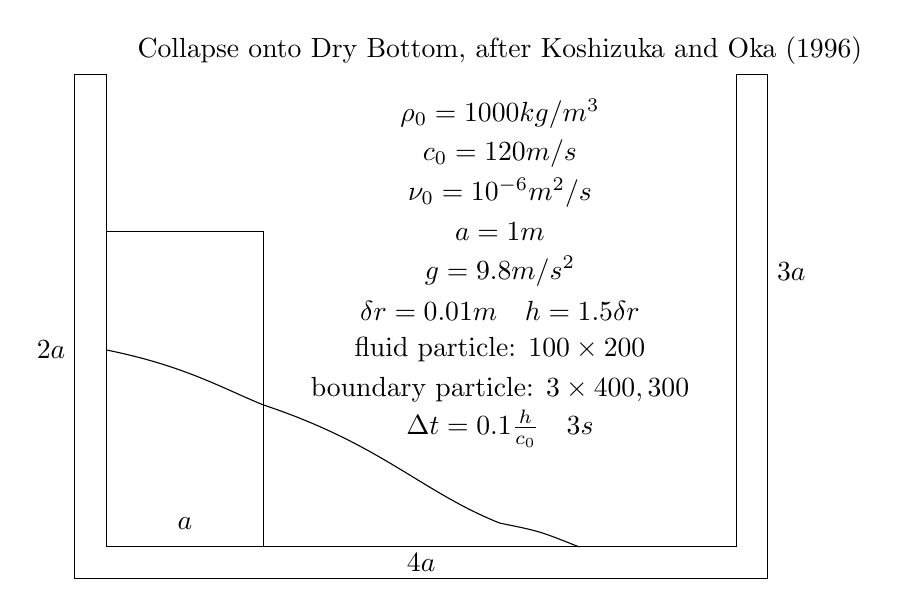
\begin{tikzpicture}
            \draw[-] (0,6)--(0,0)--(8,0)--(8,6);
            \draw[-] (0,6)--(-0.4,6)--(-0.4,-0.4)--(8.4,-0.4)--(8.4,6)--(8,6);
            \draw[-] (0,4)--(2,4)--(2,0);
            
            % arbitrary fluid surface at some time
            \draw (0,2.5) .. controls (1,2.3) and (1.5,2.0) .. (2,1.8) .. controls (3.5,1.3) and (4,0.7) .. (5,0.3) .. controls (5.5,0.2) .. (6,0);
            
            \node at (1,0.3) {$a$};
            \node at (4, -0.2) {$4a$};
            \node at (-0.7, 2.5) {$2a$};
            \node at (8.7, 3.5) {$3a$};

            \node at (5, 6.3) {Collapse onto Dry Bottom, after Koshizuka and Oka (1996)};
            \node at (5, 5.5) {$\rho_0=1000kg/m^3$};
            \node at (5, 5) {$c_0=120m/s$};
            \node at (5, 4.5) {$\nu_0=10^{-6}m^2/s$};
            \node at (5, 4) {$a=1m$};
            \node at (5, 3.5) {$g=9.8m/s^2$};
            \node at (5, 3) {$\delta r=0.01m\quad h=1.5\delta r$};
            \node at (5, 2.5) {fluid particle: $100\times 200$};
            \node at (5, 2) {boundary particle: $3\times 400,300$};
            \node at (5, 1.5) {$\Delta t=0.1\frac{h}{c_0}\quad 3s$};
        \end{tikzpicture}
    \end{figure}
\end{frame}

\begin{frame}
    \begin{figure}[H]
        \centering
        \subfigure[壁面粒子未垫高]{
            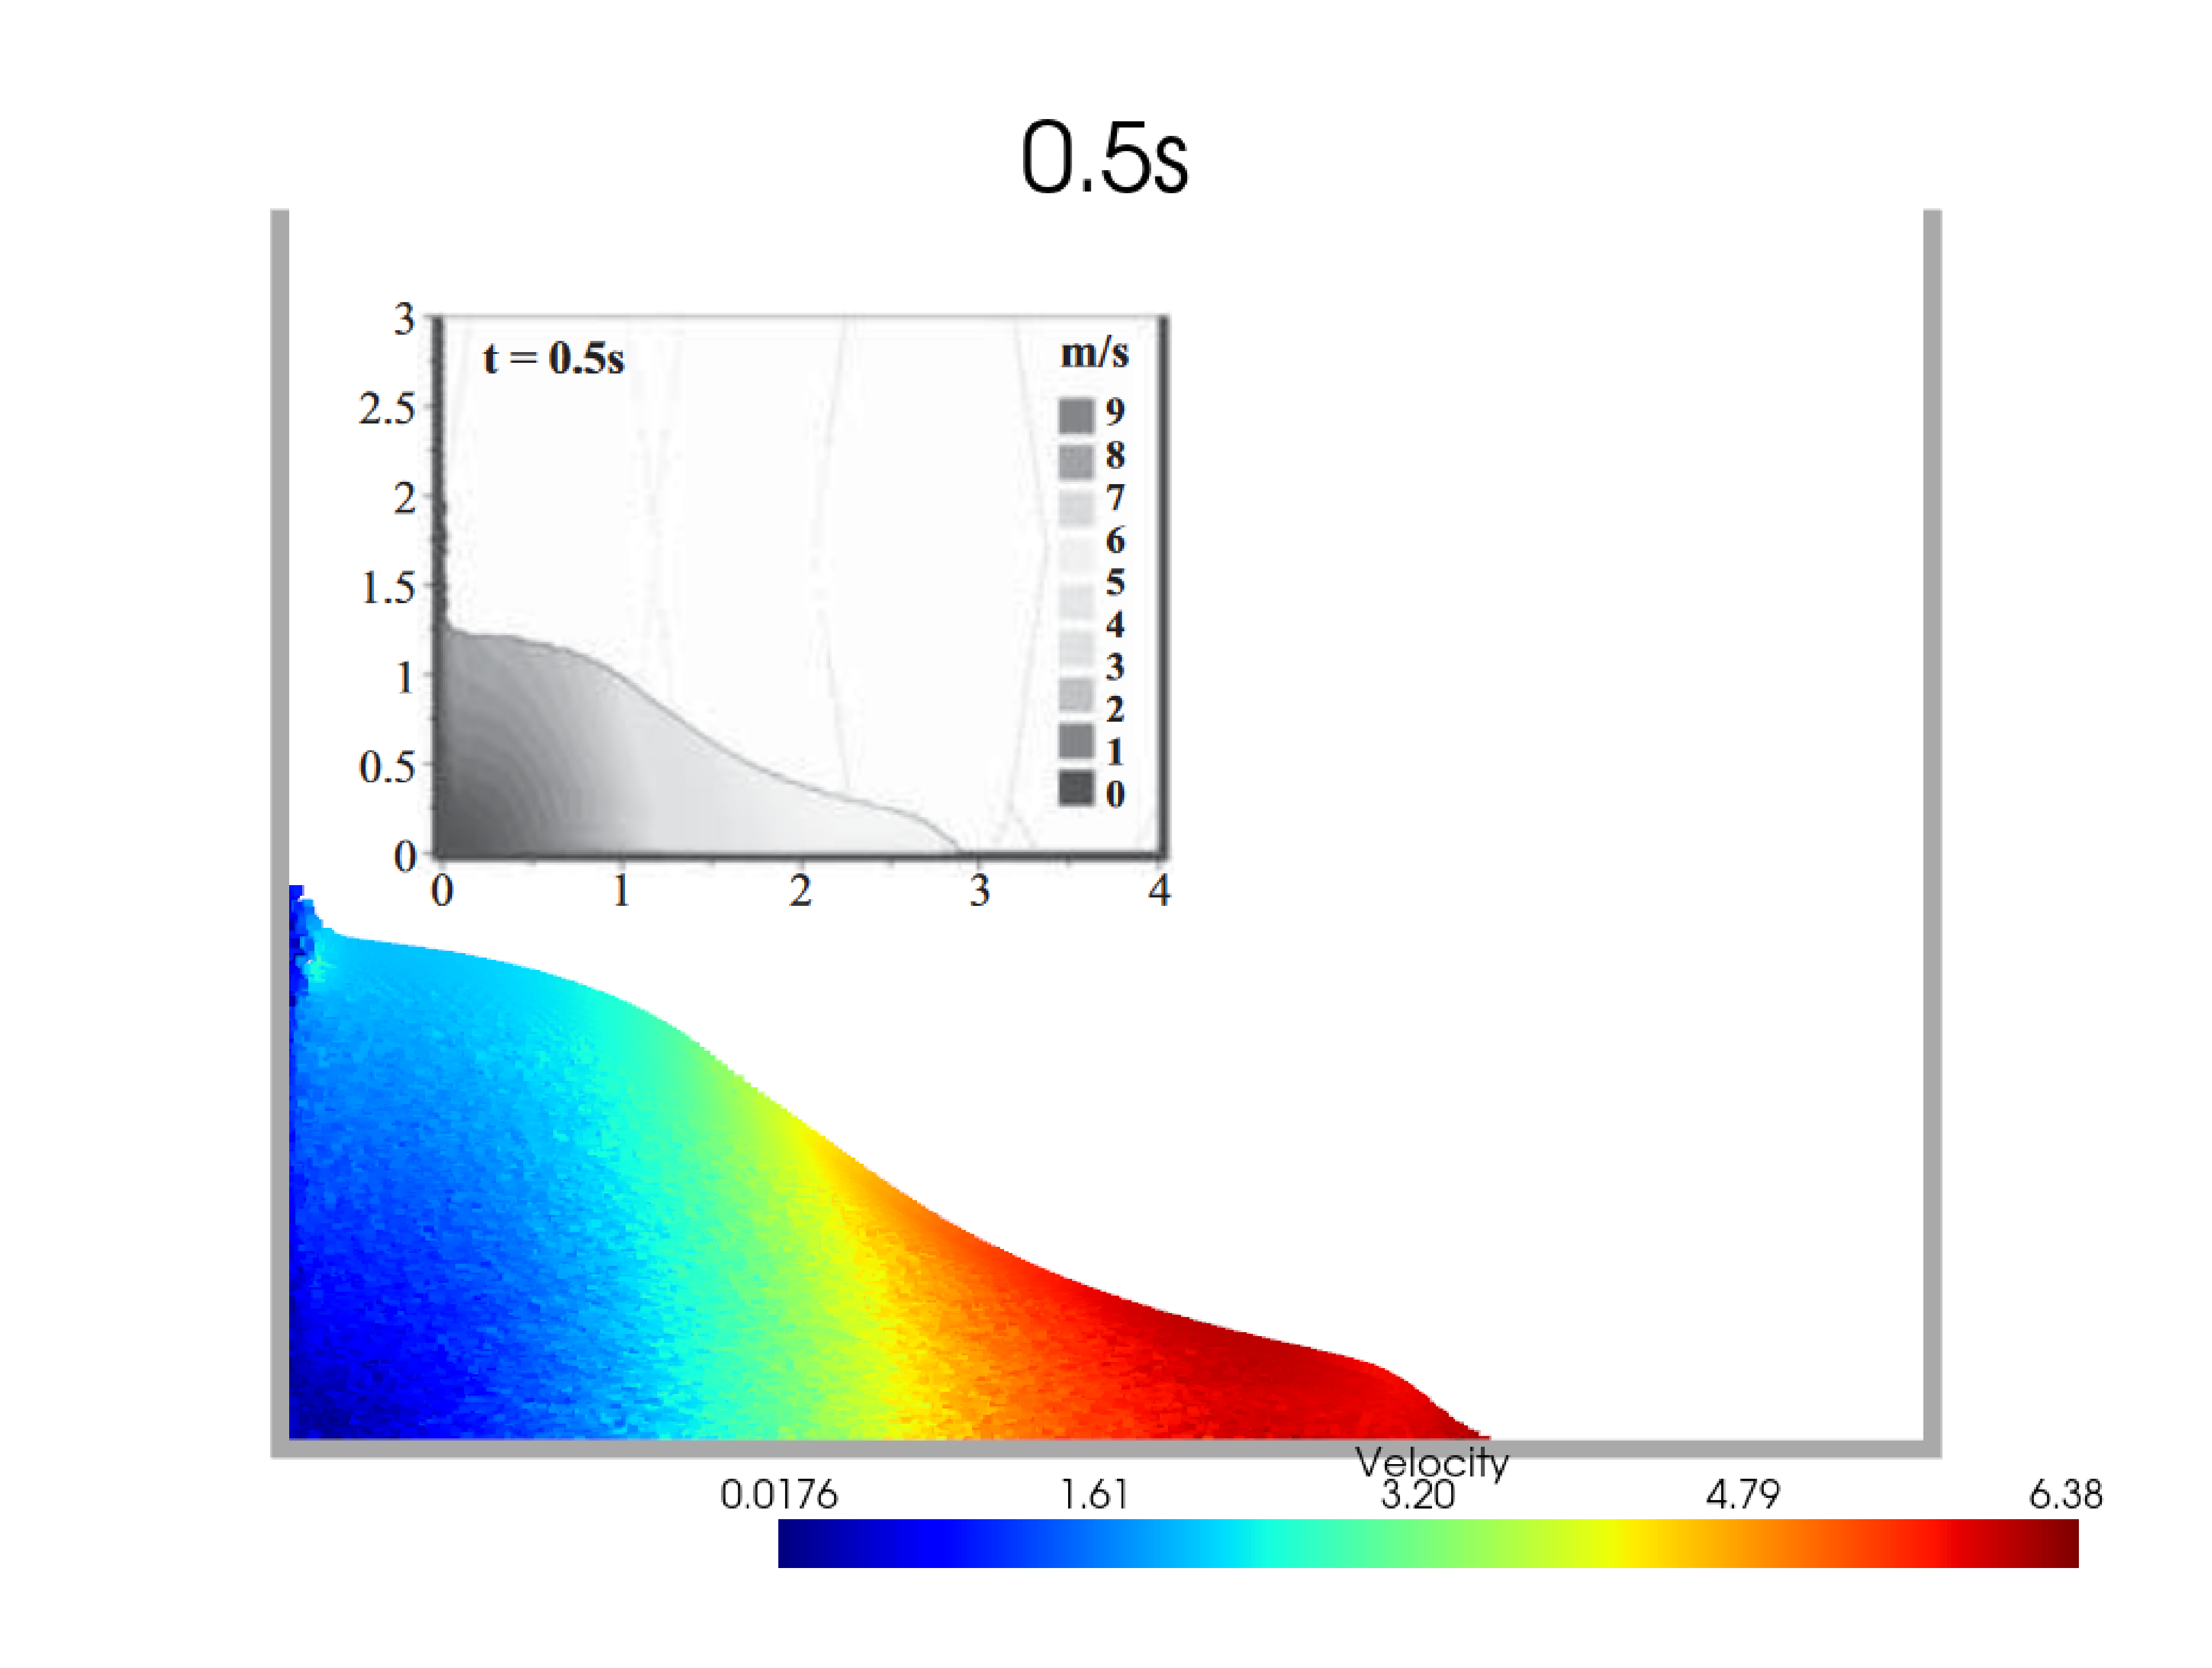
\includegraphics[width=0.47\textwidth]{images/CollapseDry/origin/collapse_dry05_combined.png}
        }
        \subfigure[壁面粒子垫高]{
            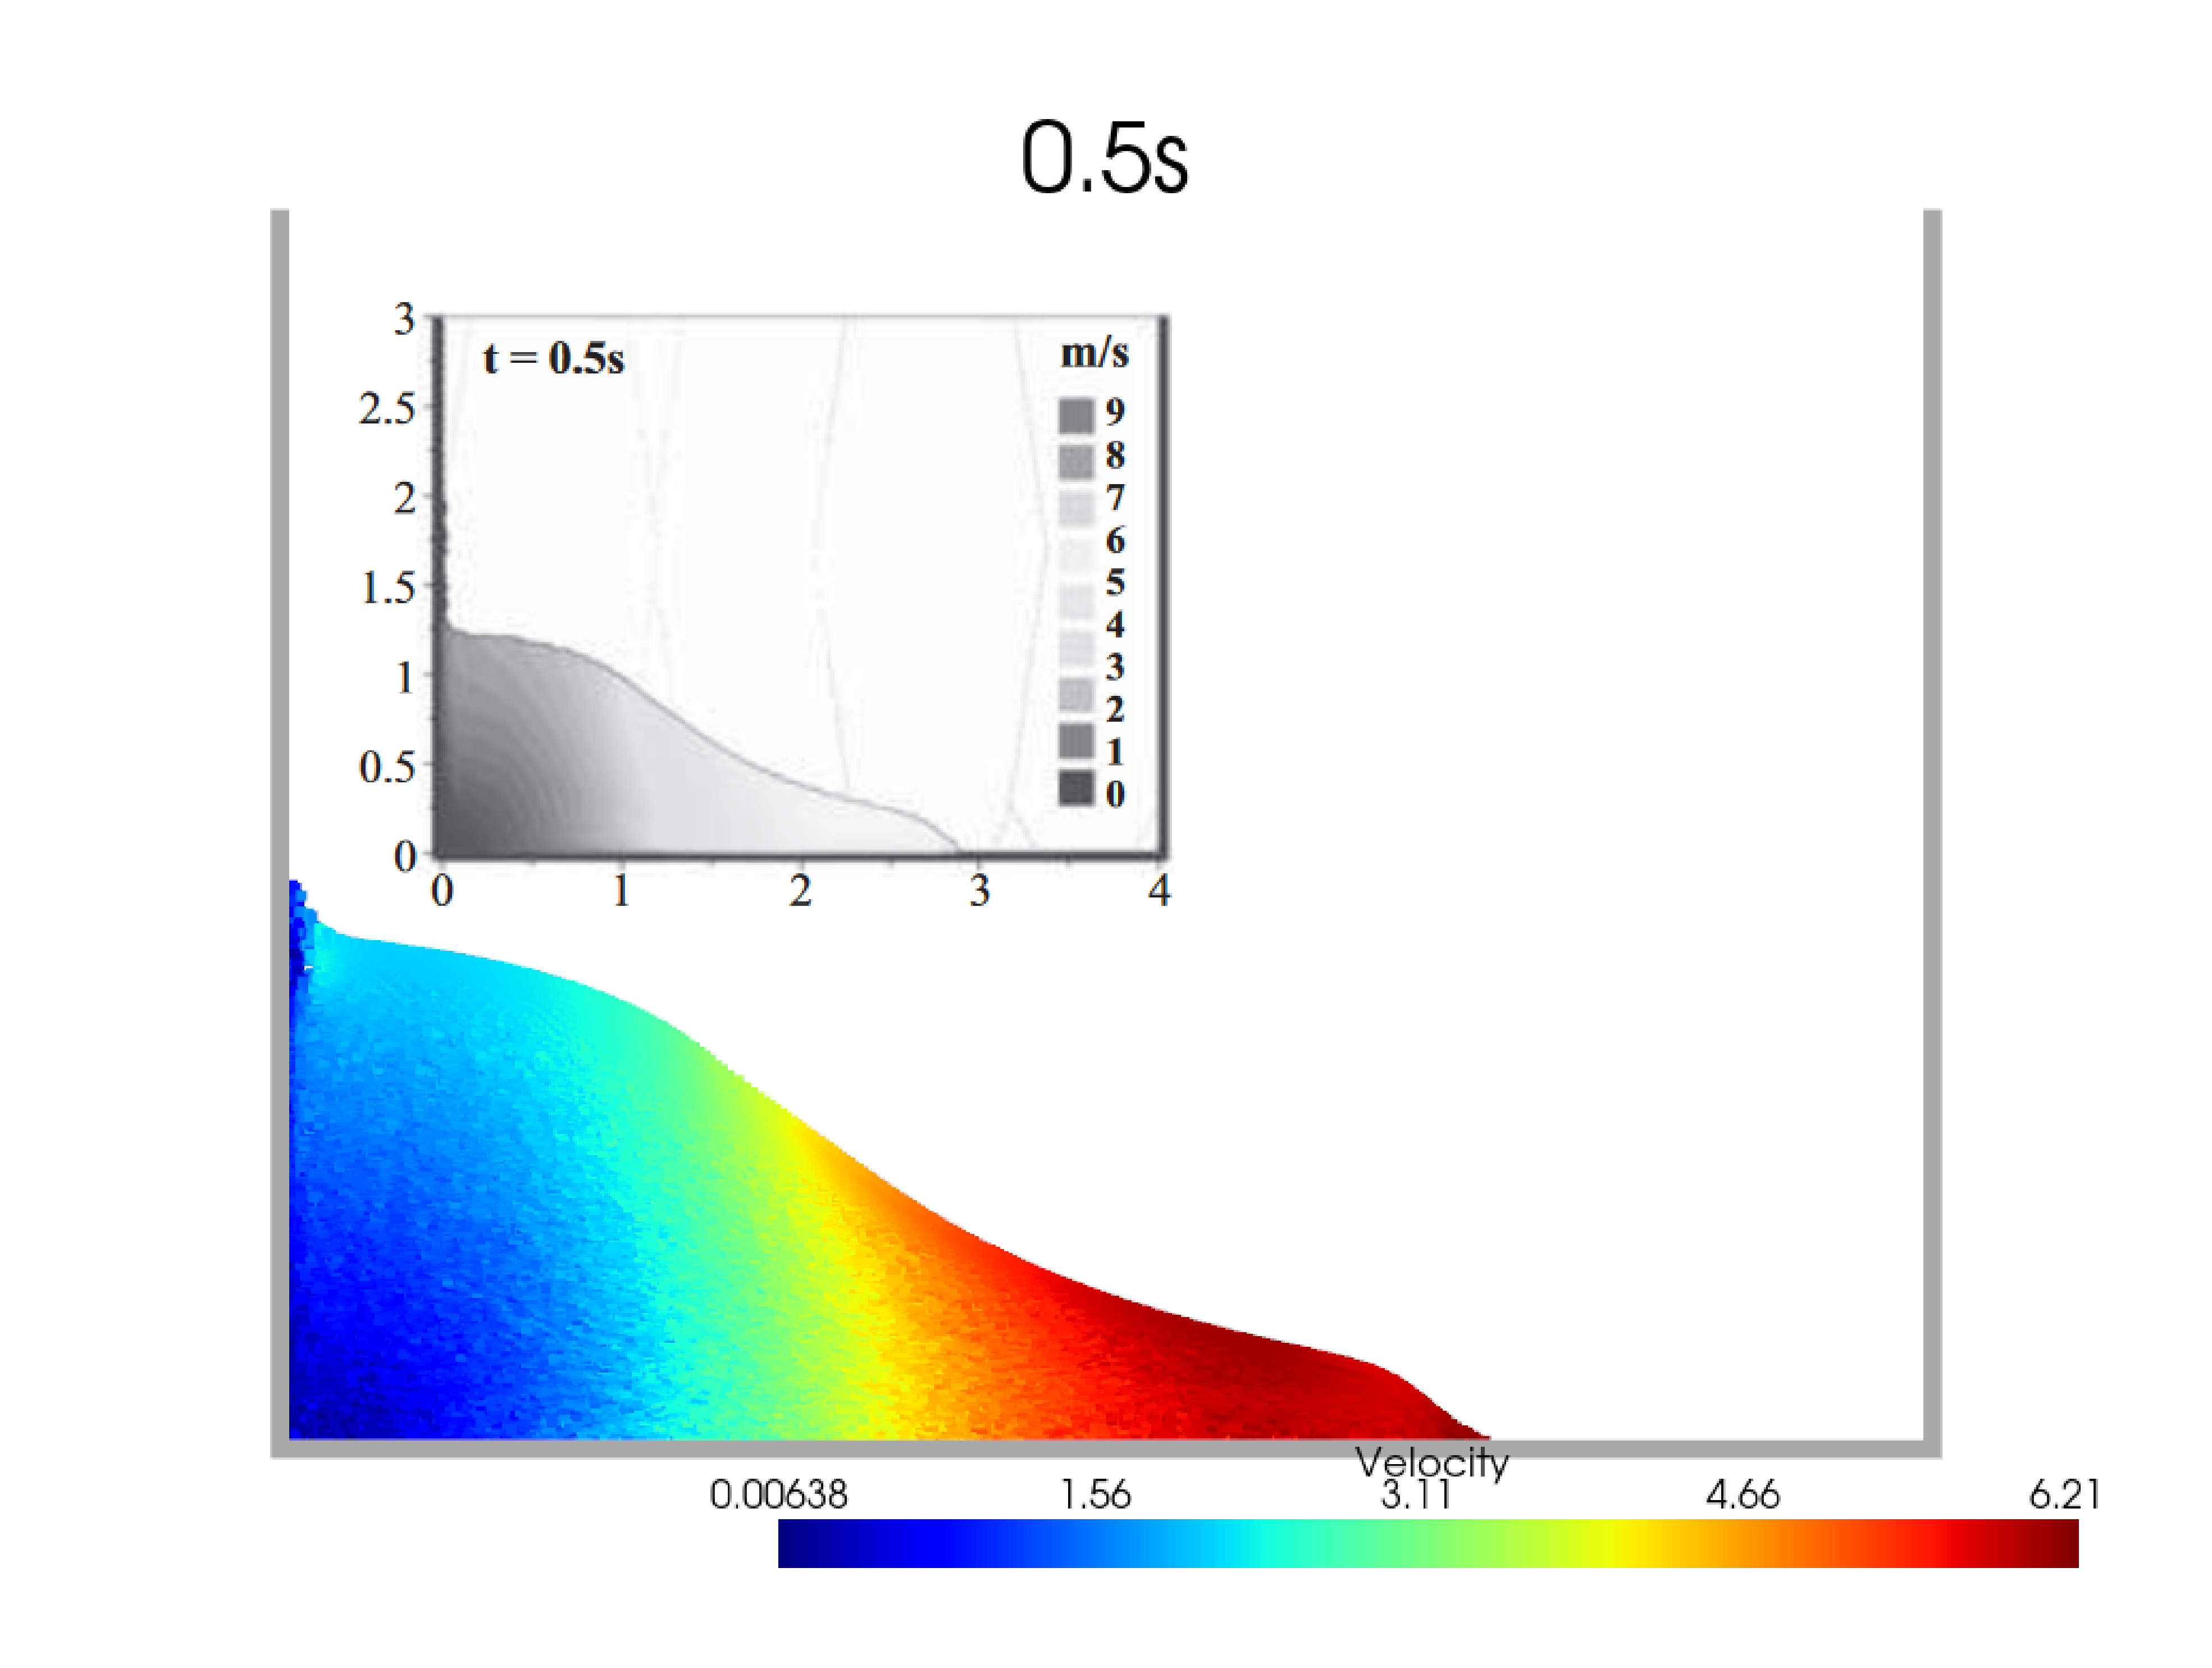
\includegraphics[width=0.47\textwidth]{images/CollapseDry/half/collapse_dry05_combined.png}
        }
    \end{figure}
\end{frame}

\begin{frame}
    \begin{figure}[H]
        \centering
        \subfigure[壁面粒子未垫高]{
            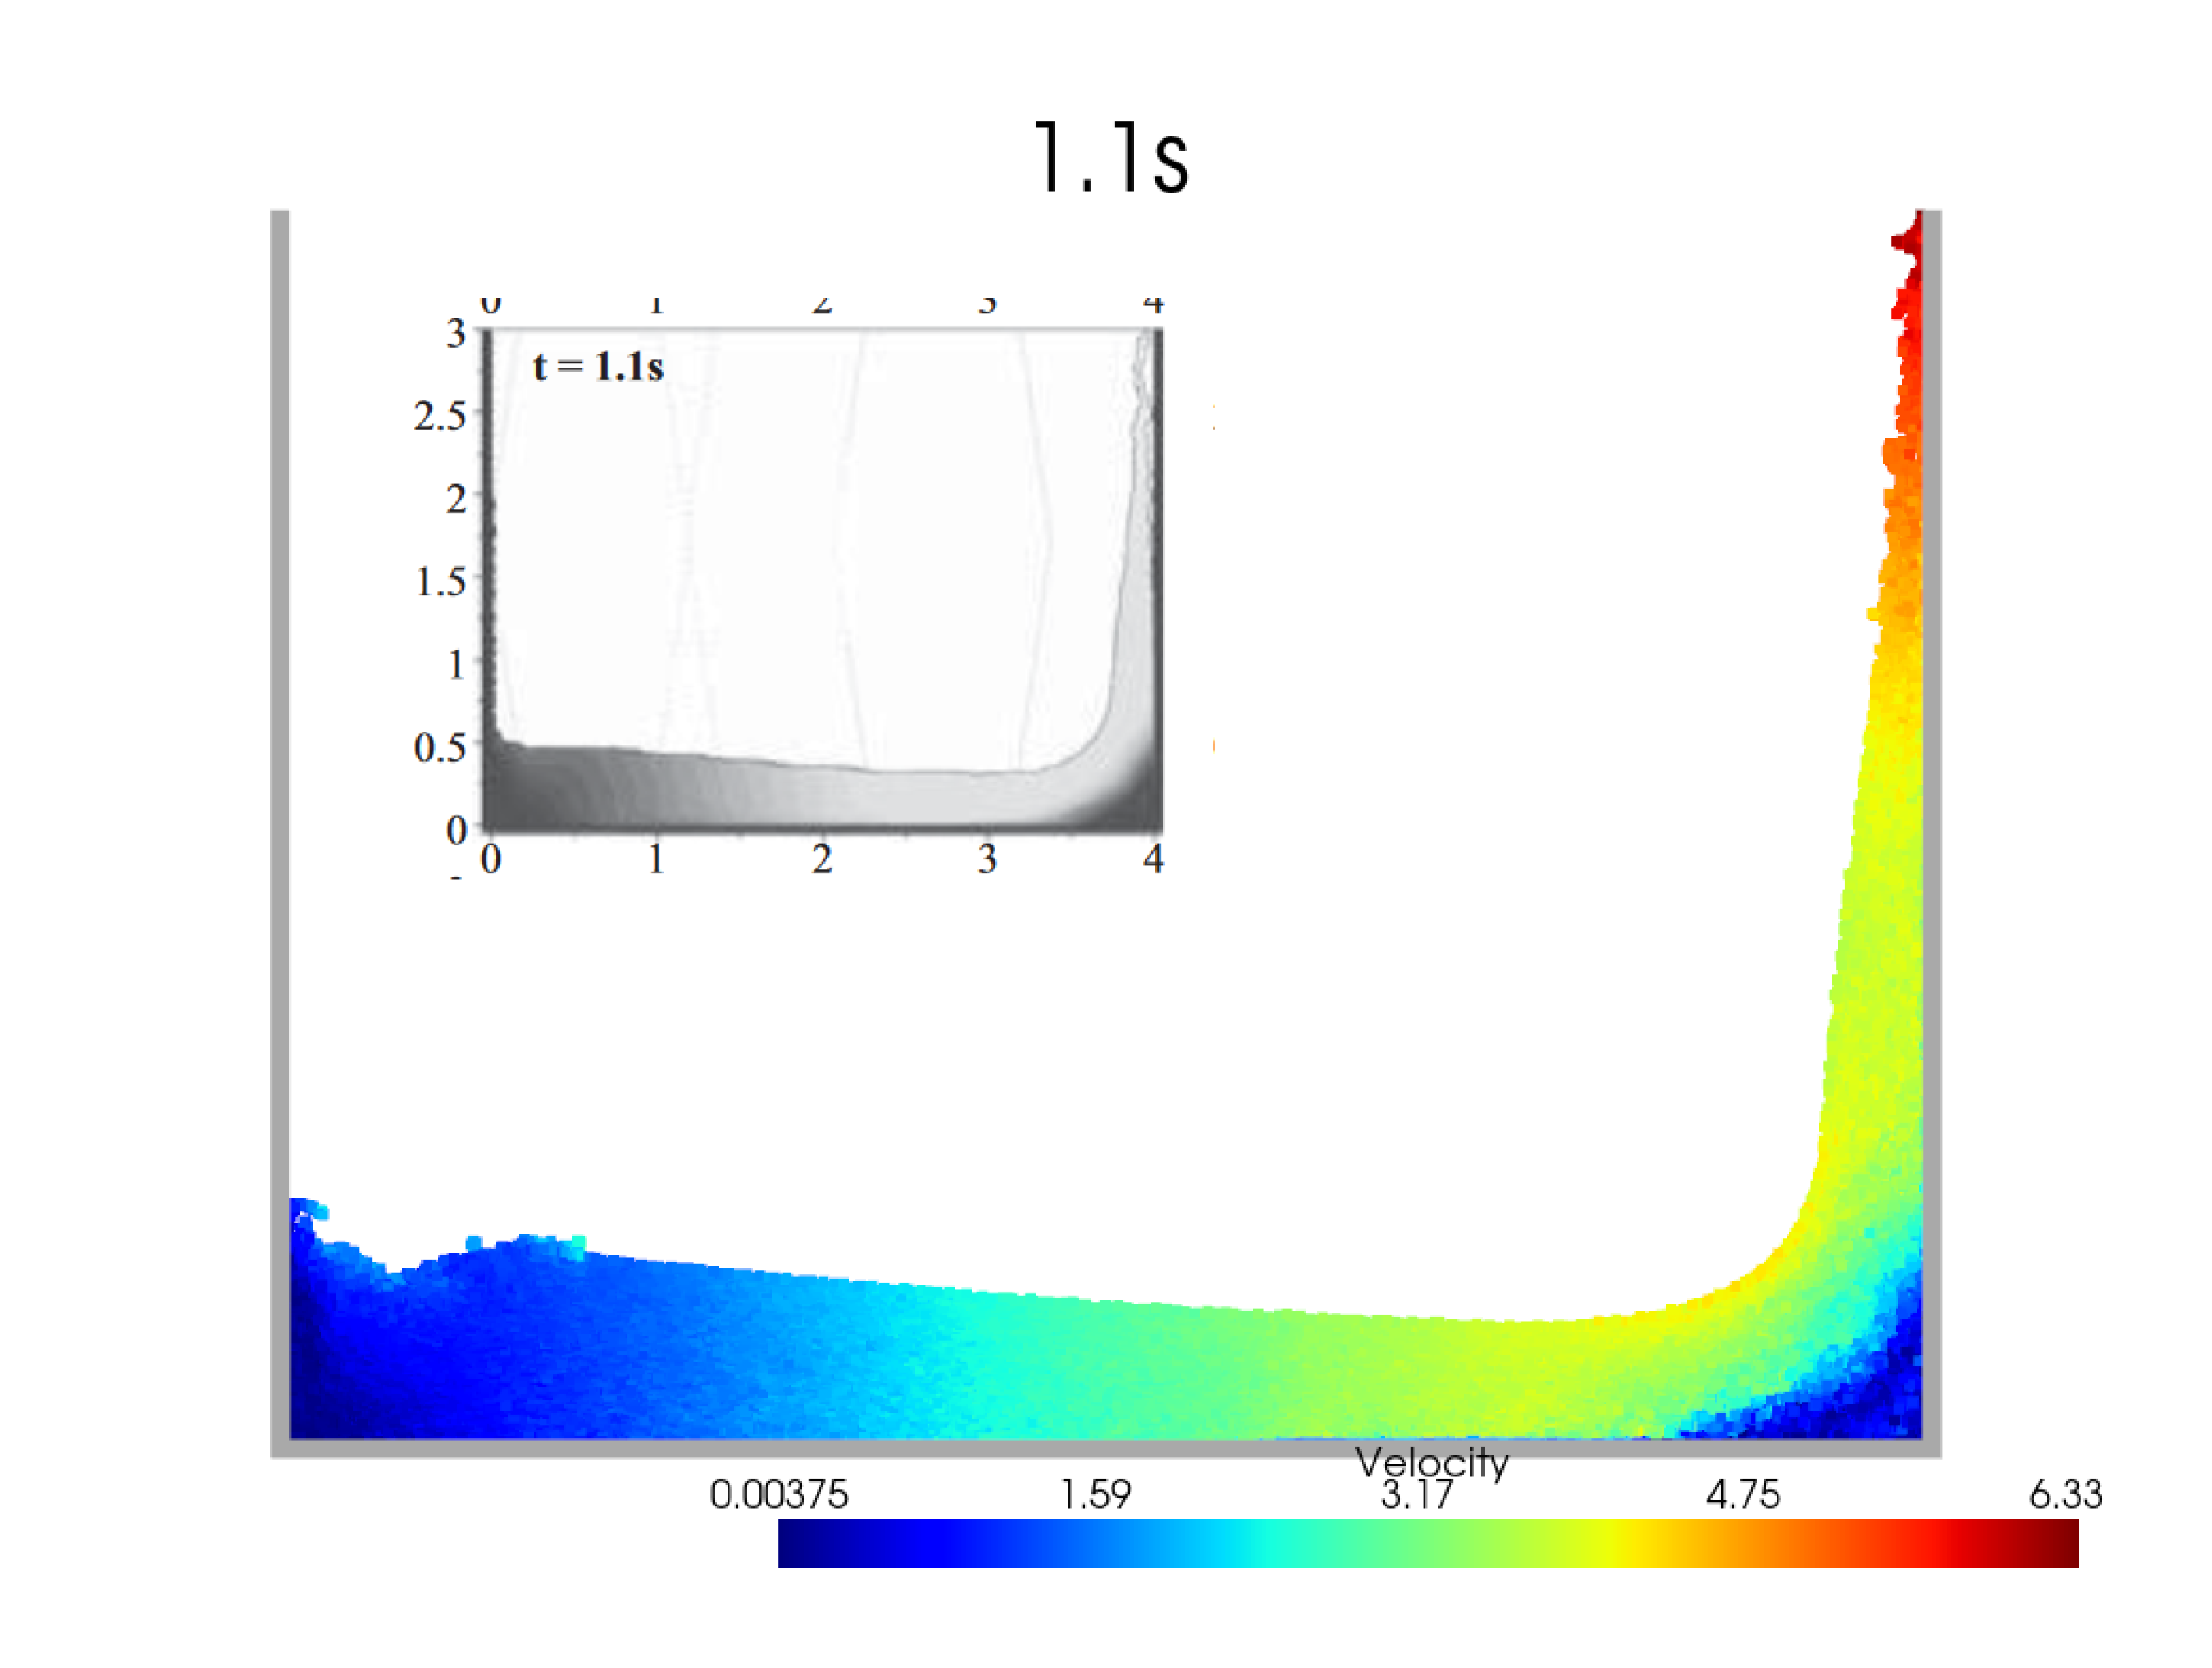
\includegraphics[width=0.47\textwidth]{images/CollapseDry/origin/collapse_dry11_combined.png}
        }
        \subfigure[壁面粒子垫高]{
            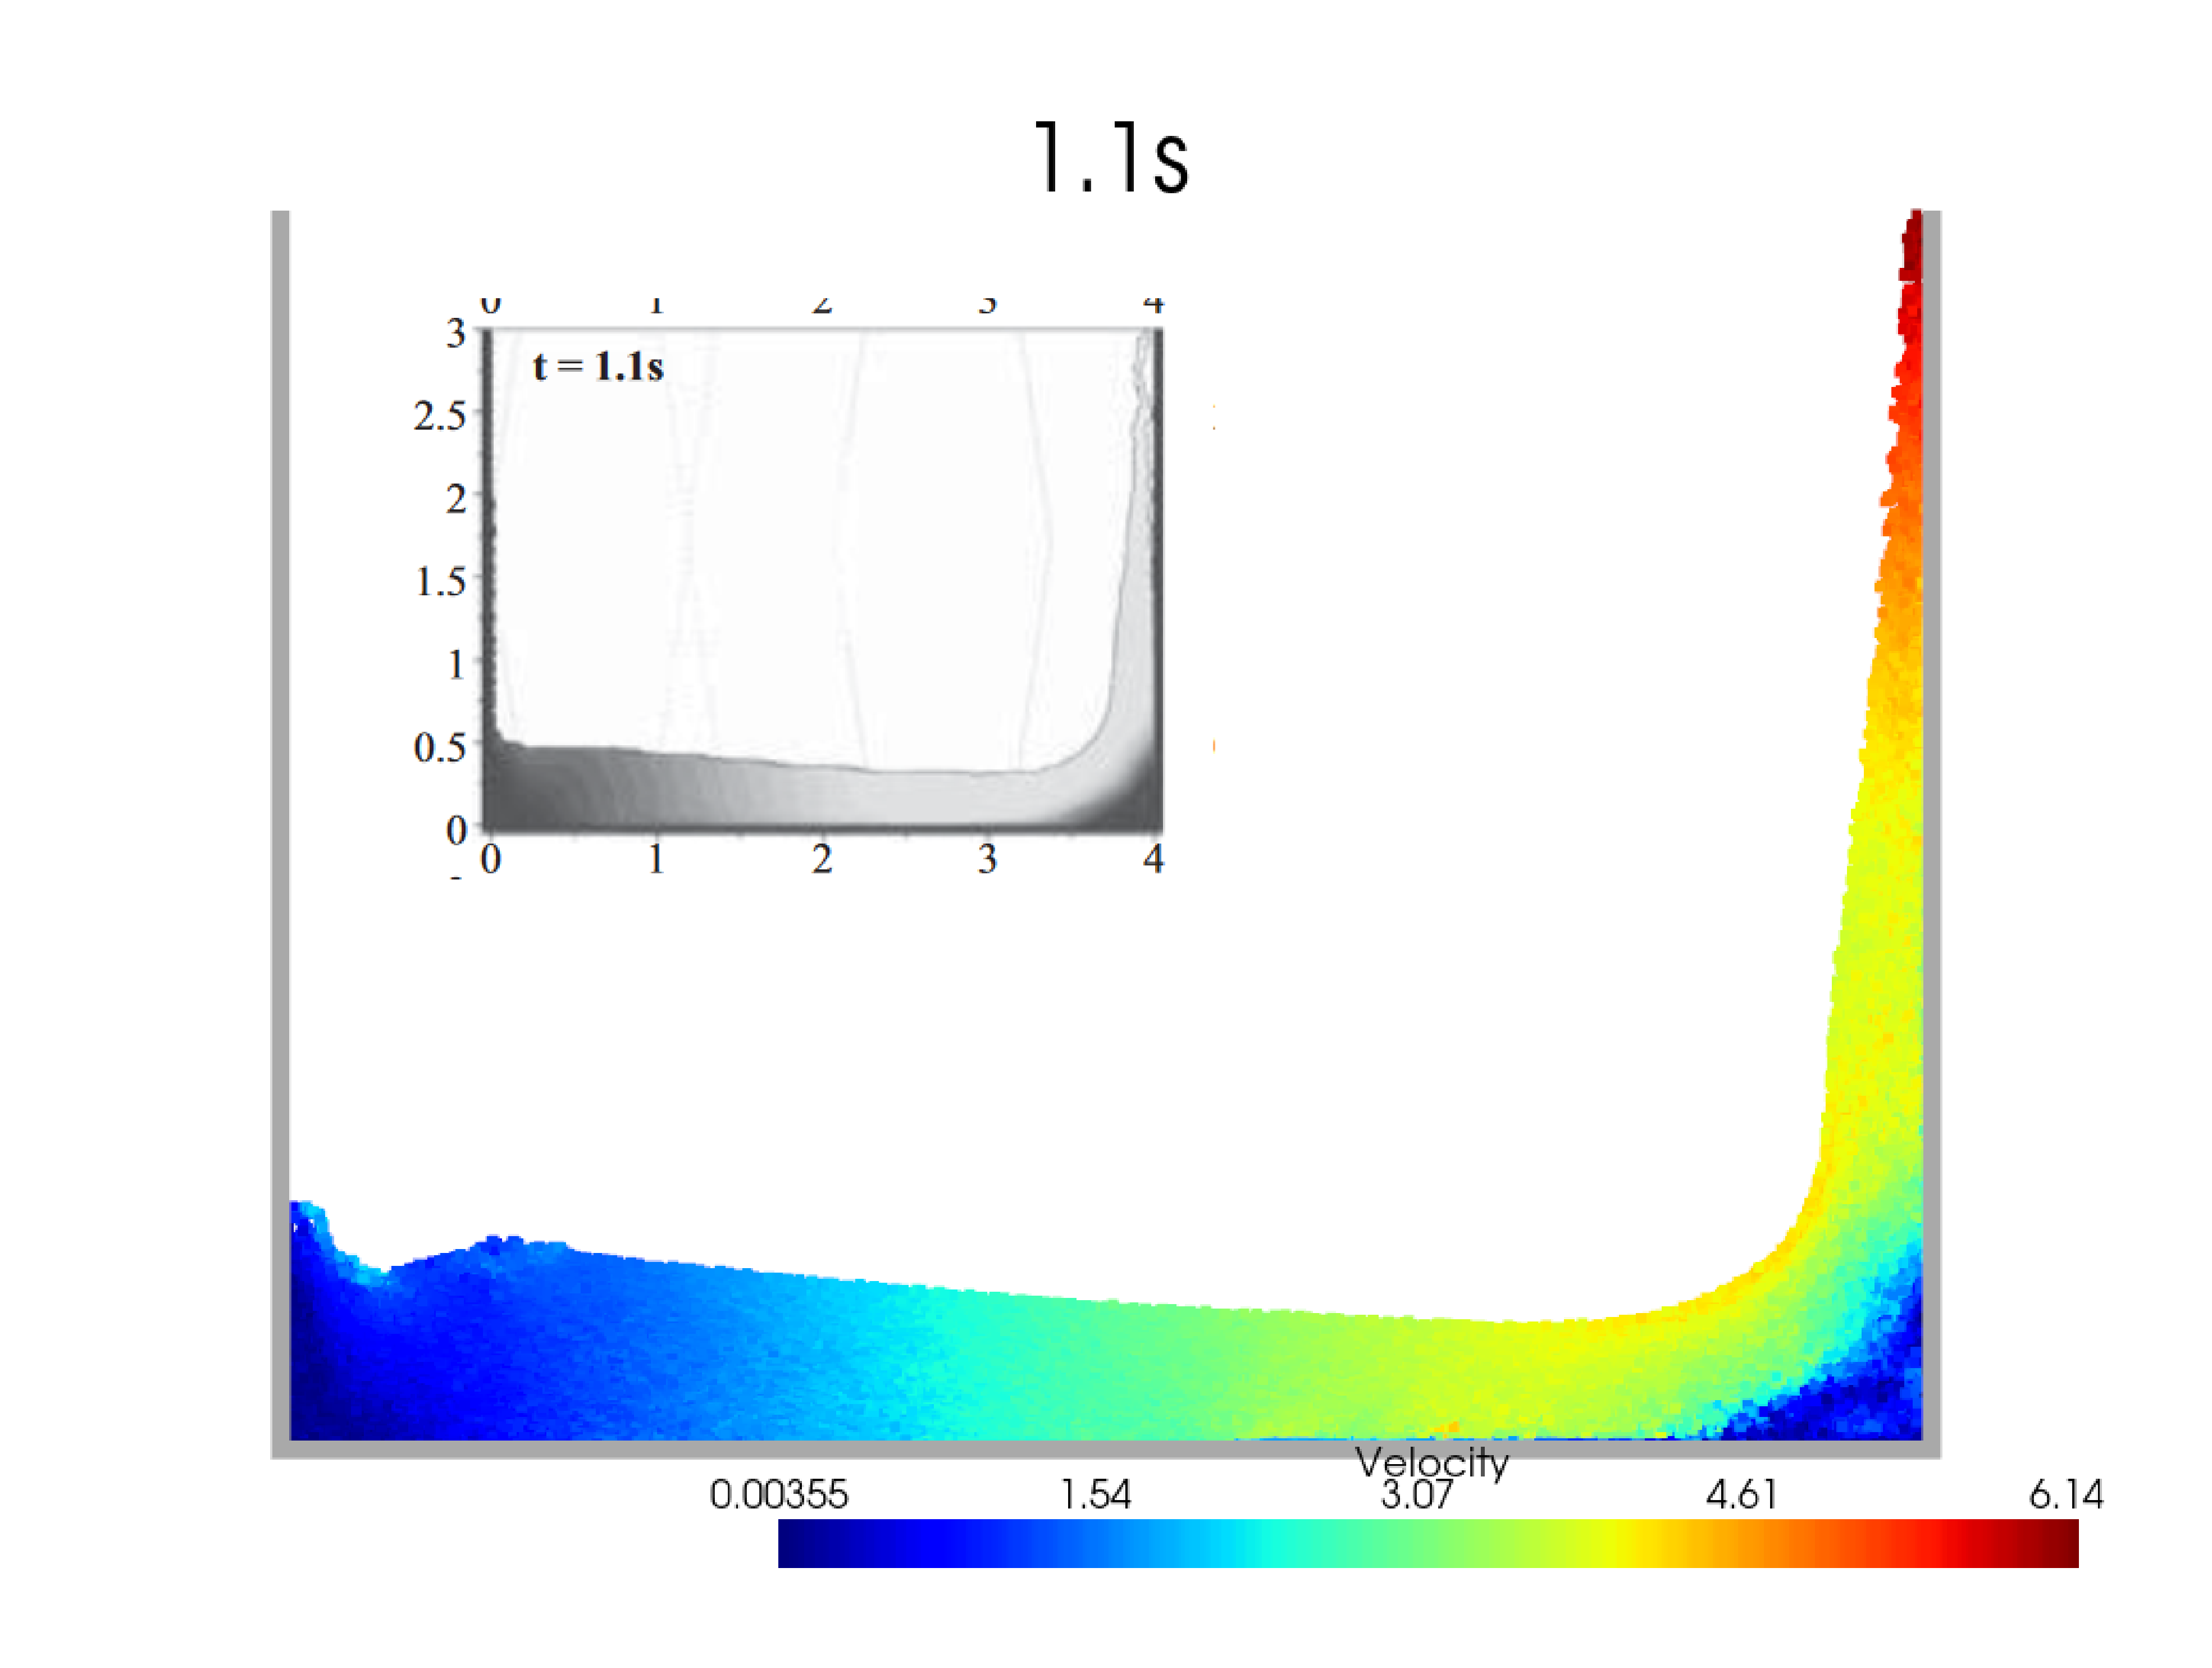
\includegraphics[width=0.47\textwidth]{images/CollapseDry/half/collapse_dry11_combined.png}
        }
    \end{figure}
\end{frame}

\begin{frame}
    \begin{figure}[H]
        \centering
        \subfigure[壁面粒子未垫高]{
            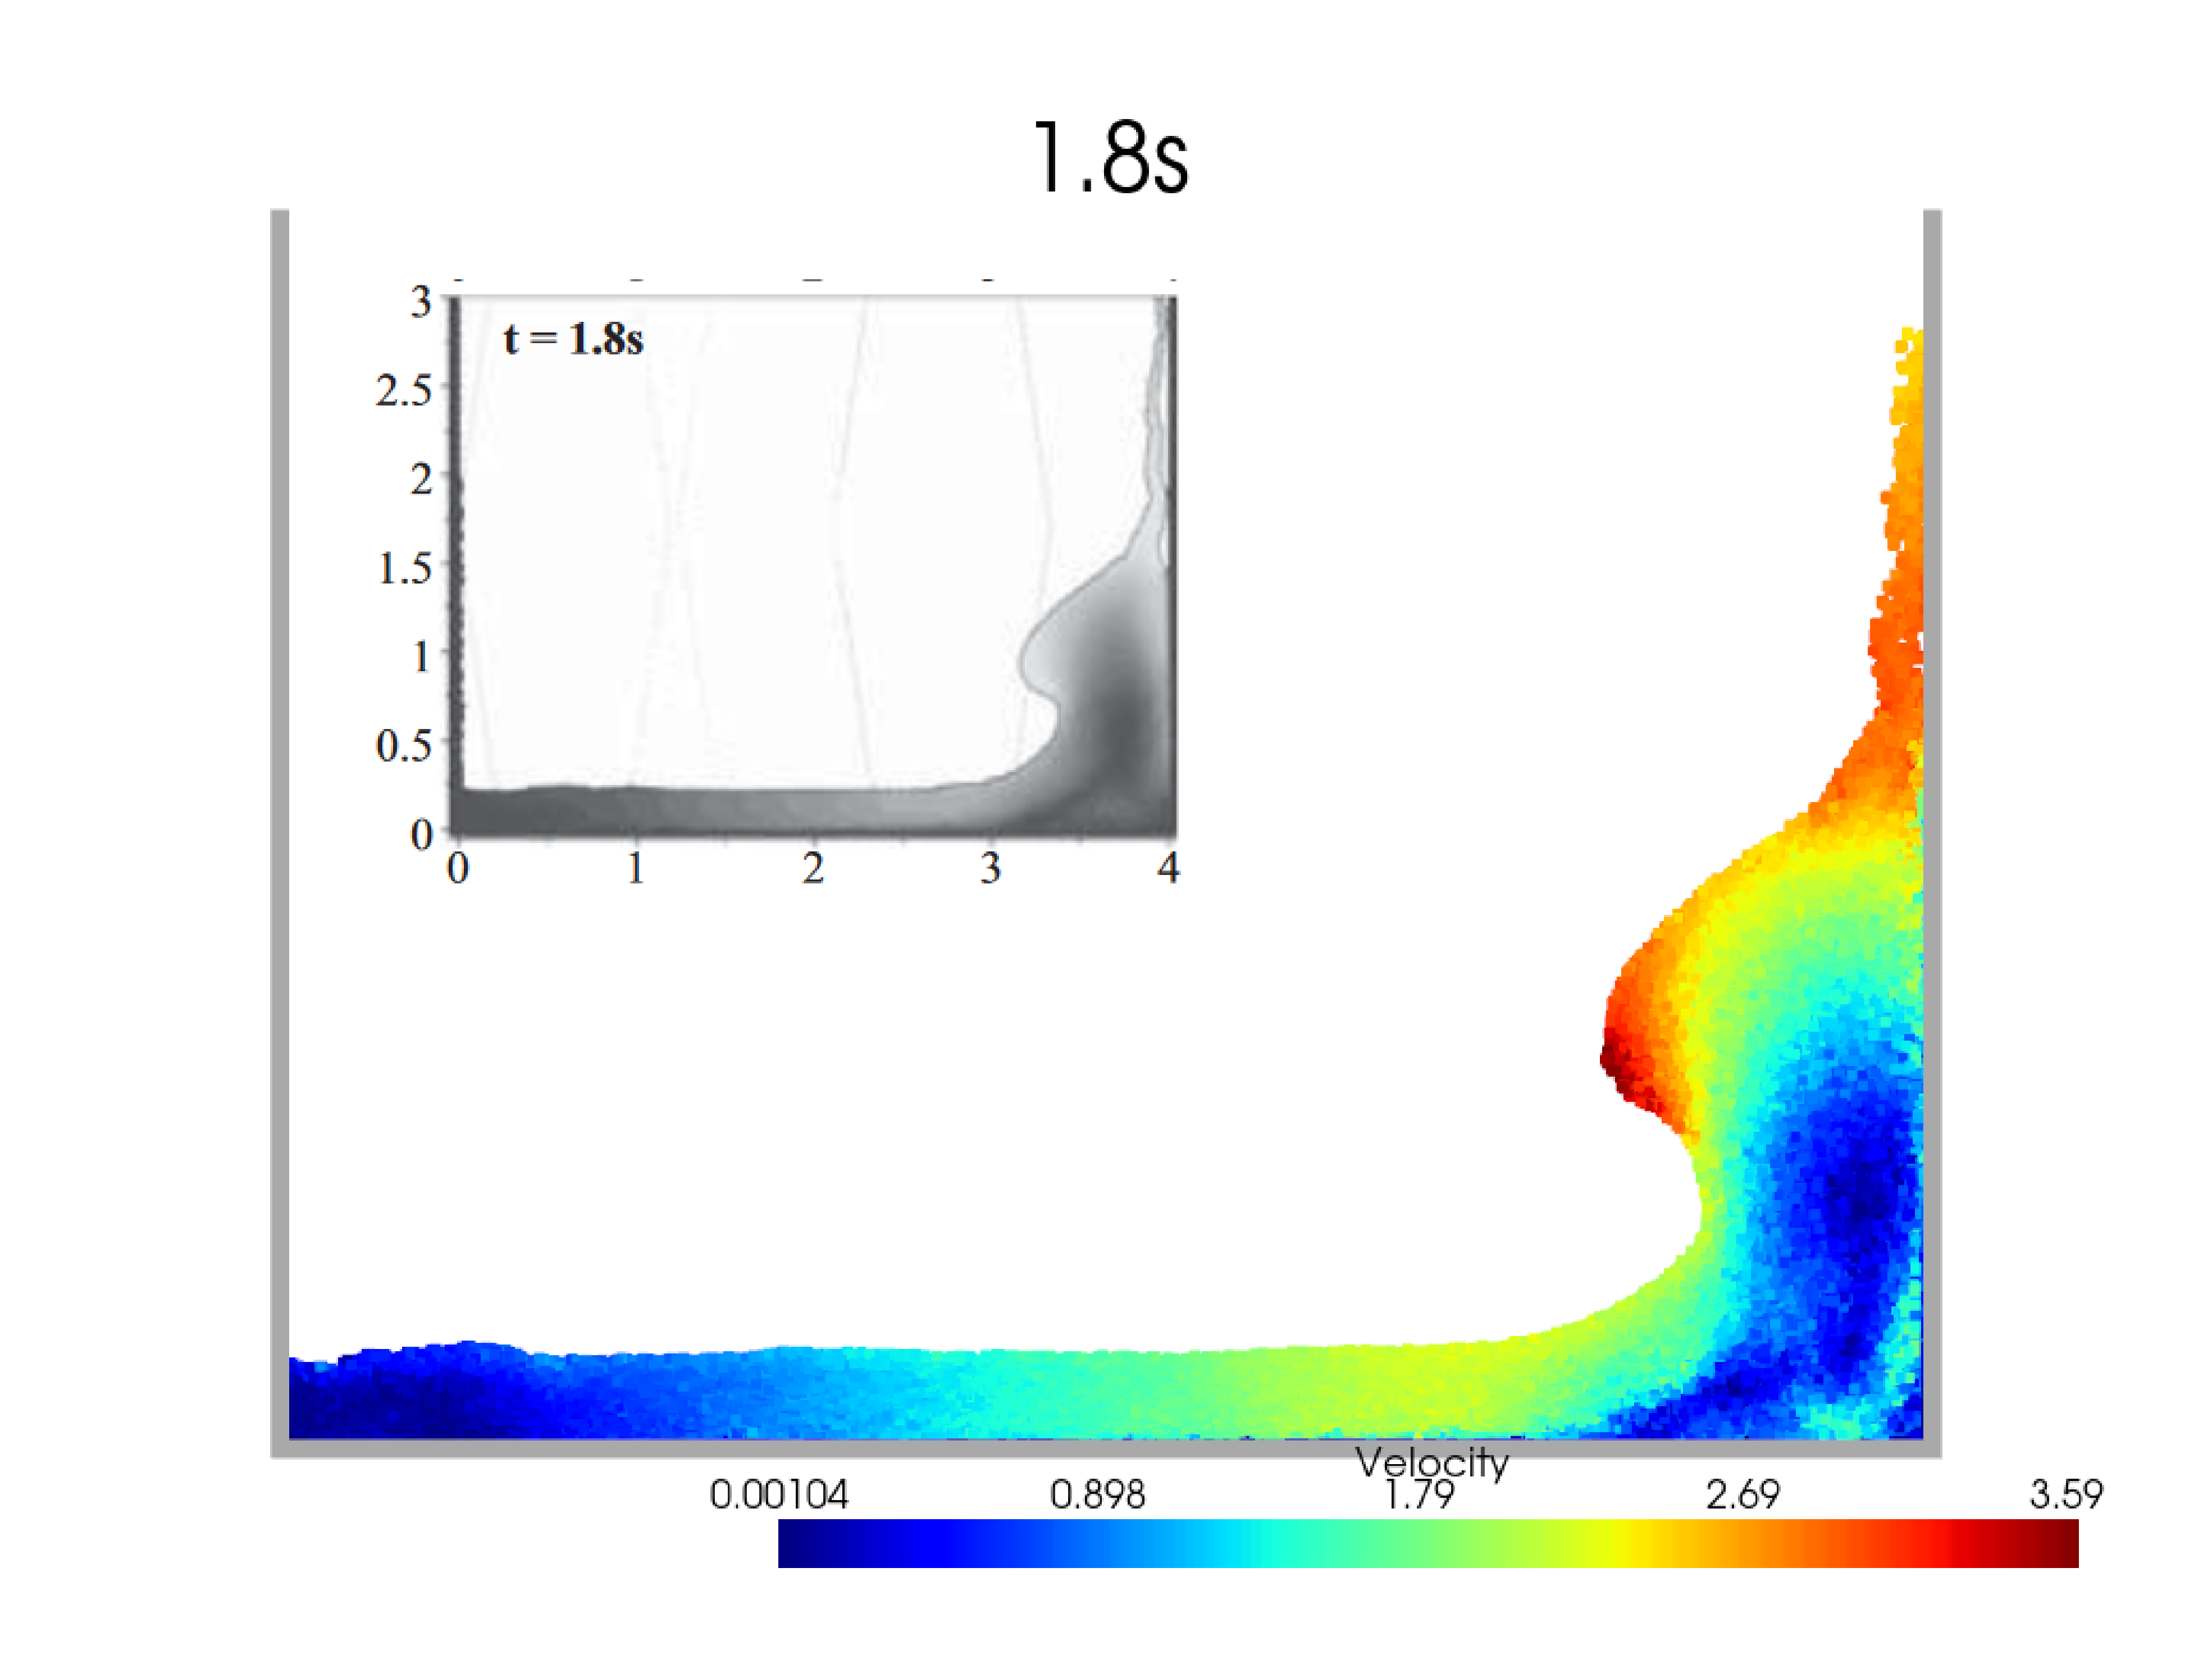
\includegraphics[width=0.47\textwidth]{images/CollapseDry/origin/collapse_dry18_combined.png}
        }
        \subfigure[壁面粒子垫高]{
            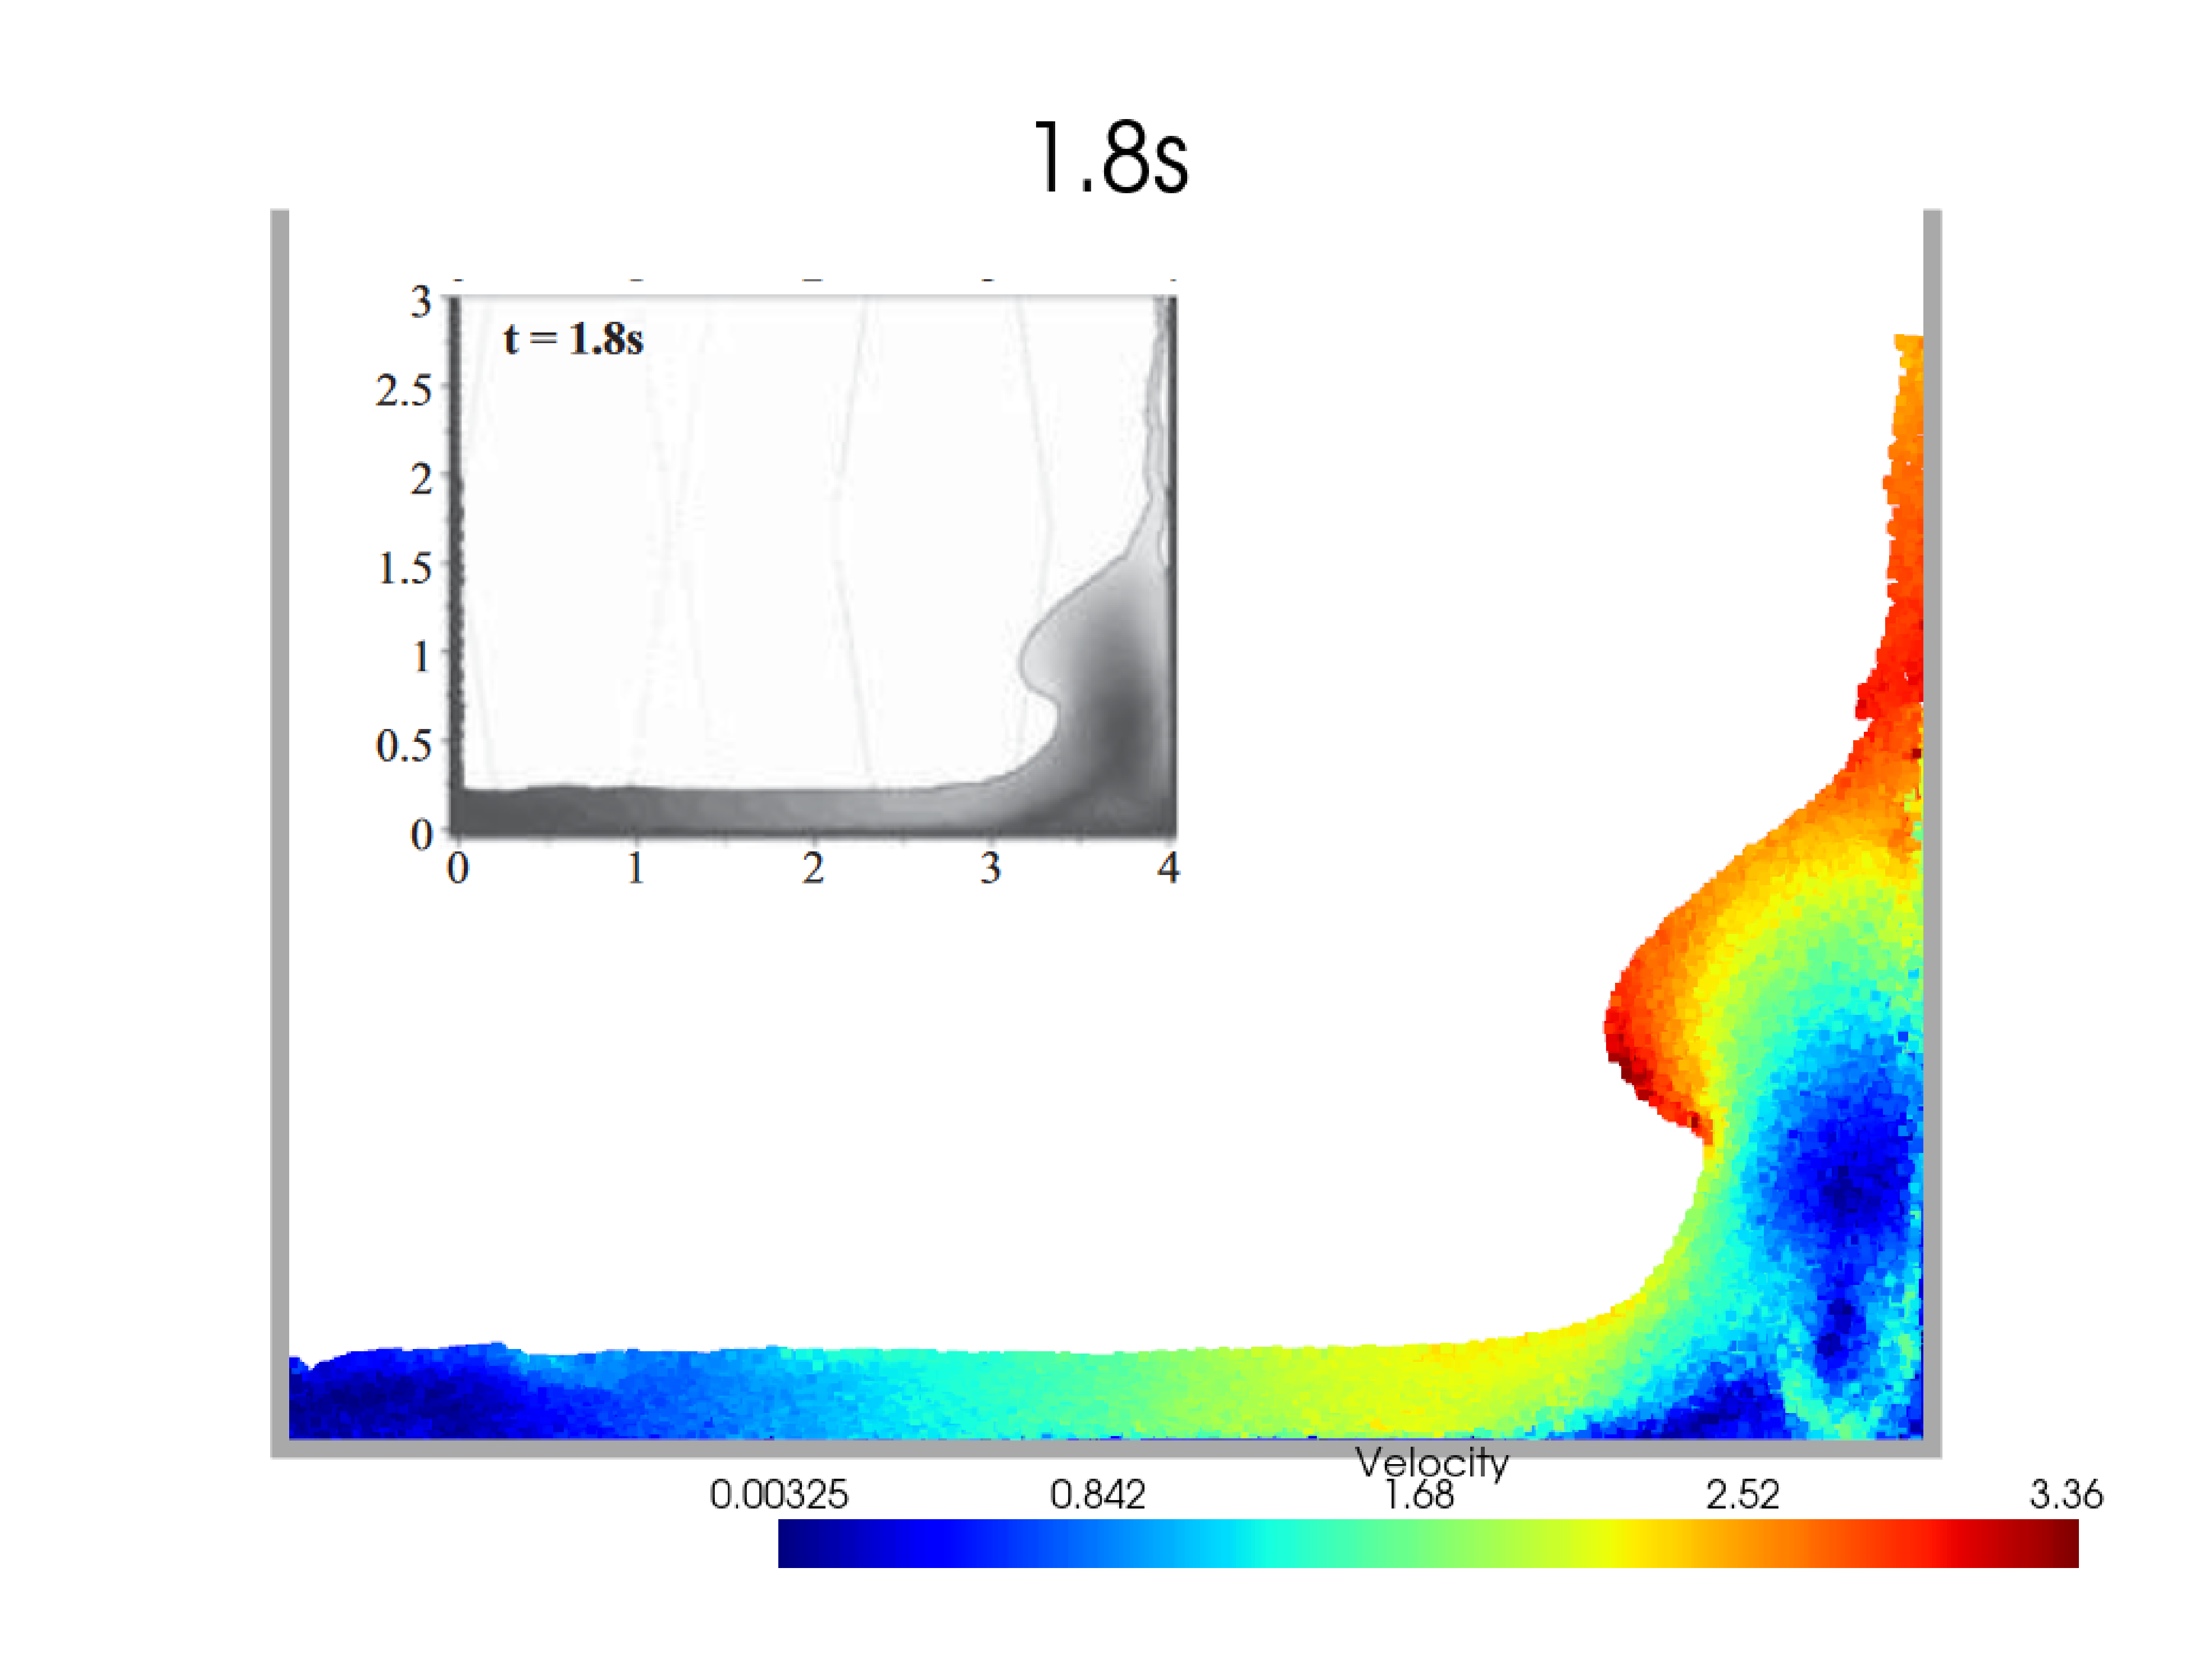
\includegraphics[width=0.47\textwidth]{images/CollapseDry/half/collapse_dry18_combined.png}
        }
    \end{figure}
\end{frame}

\begin{frame}
    \begin{figure}[H]
        \centering
        \subfigure[壁面粒子未垫高]{
            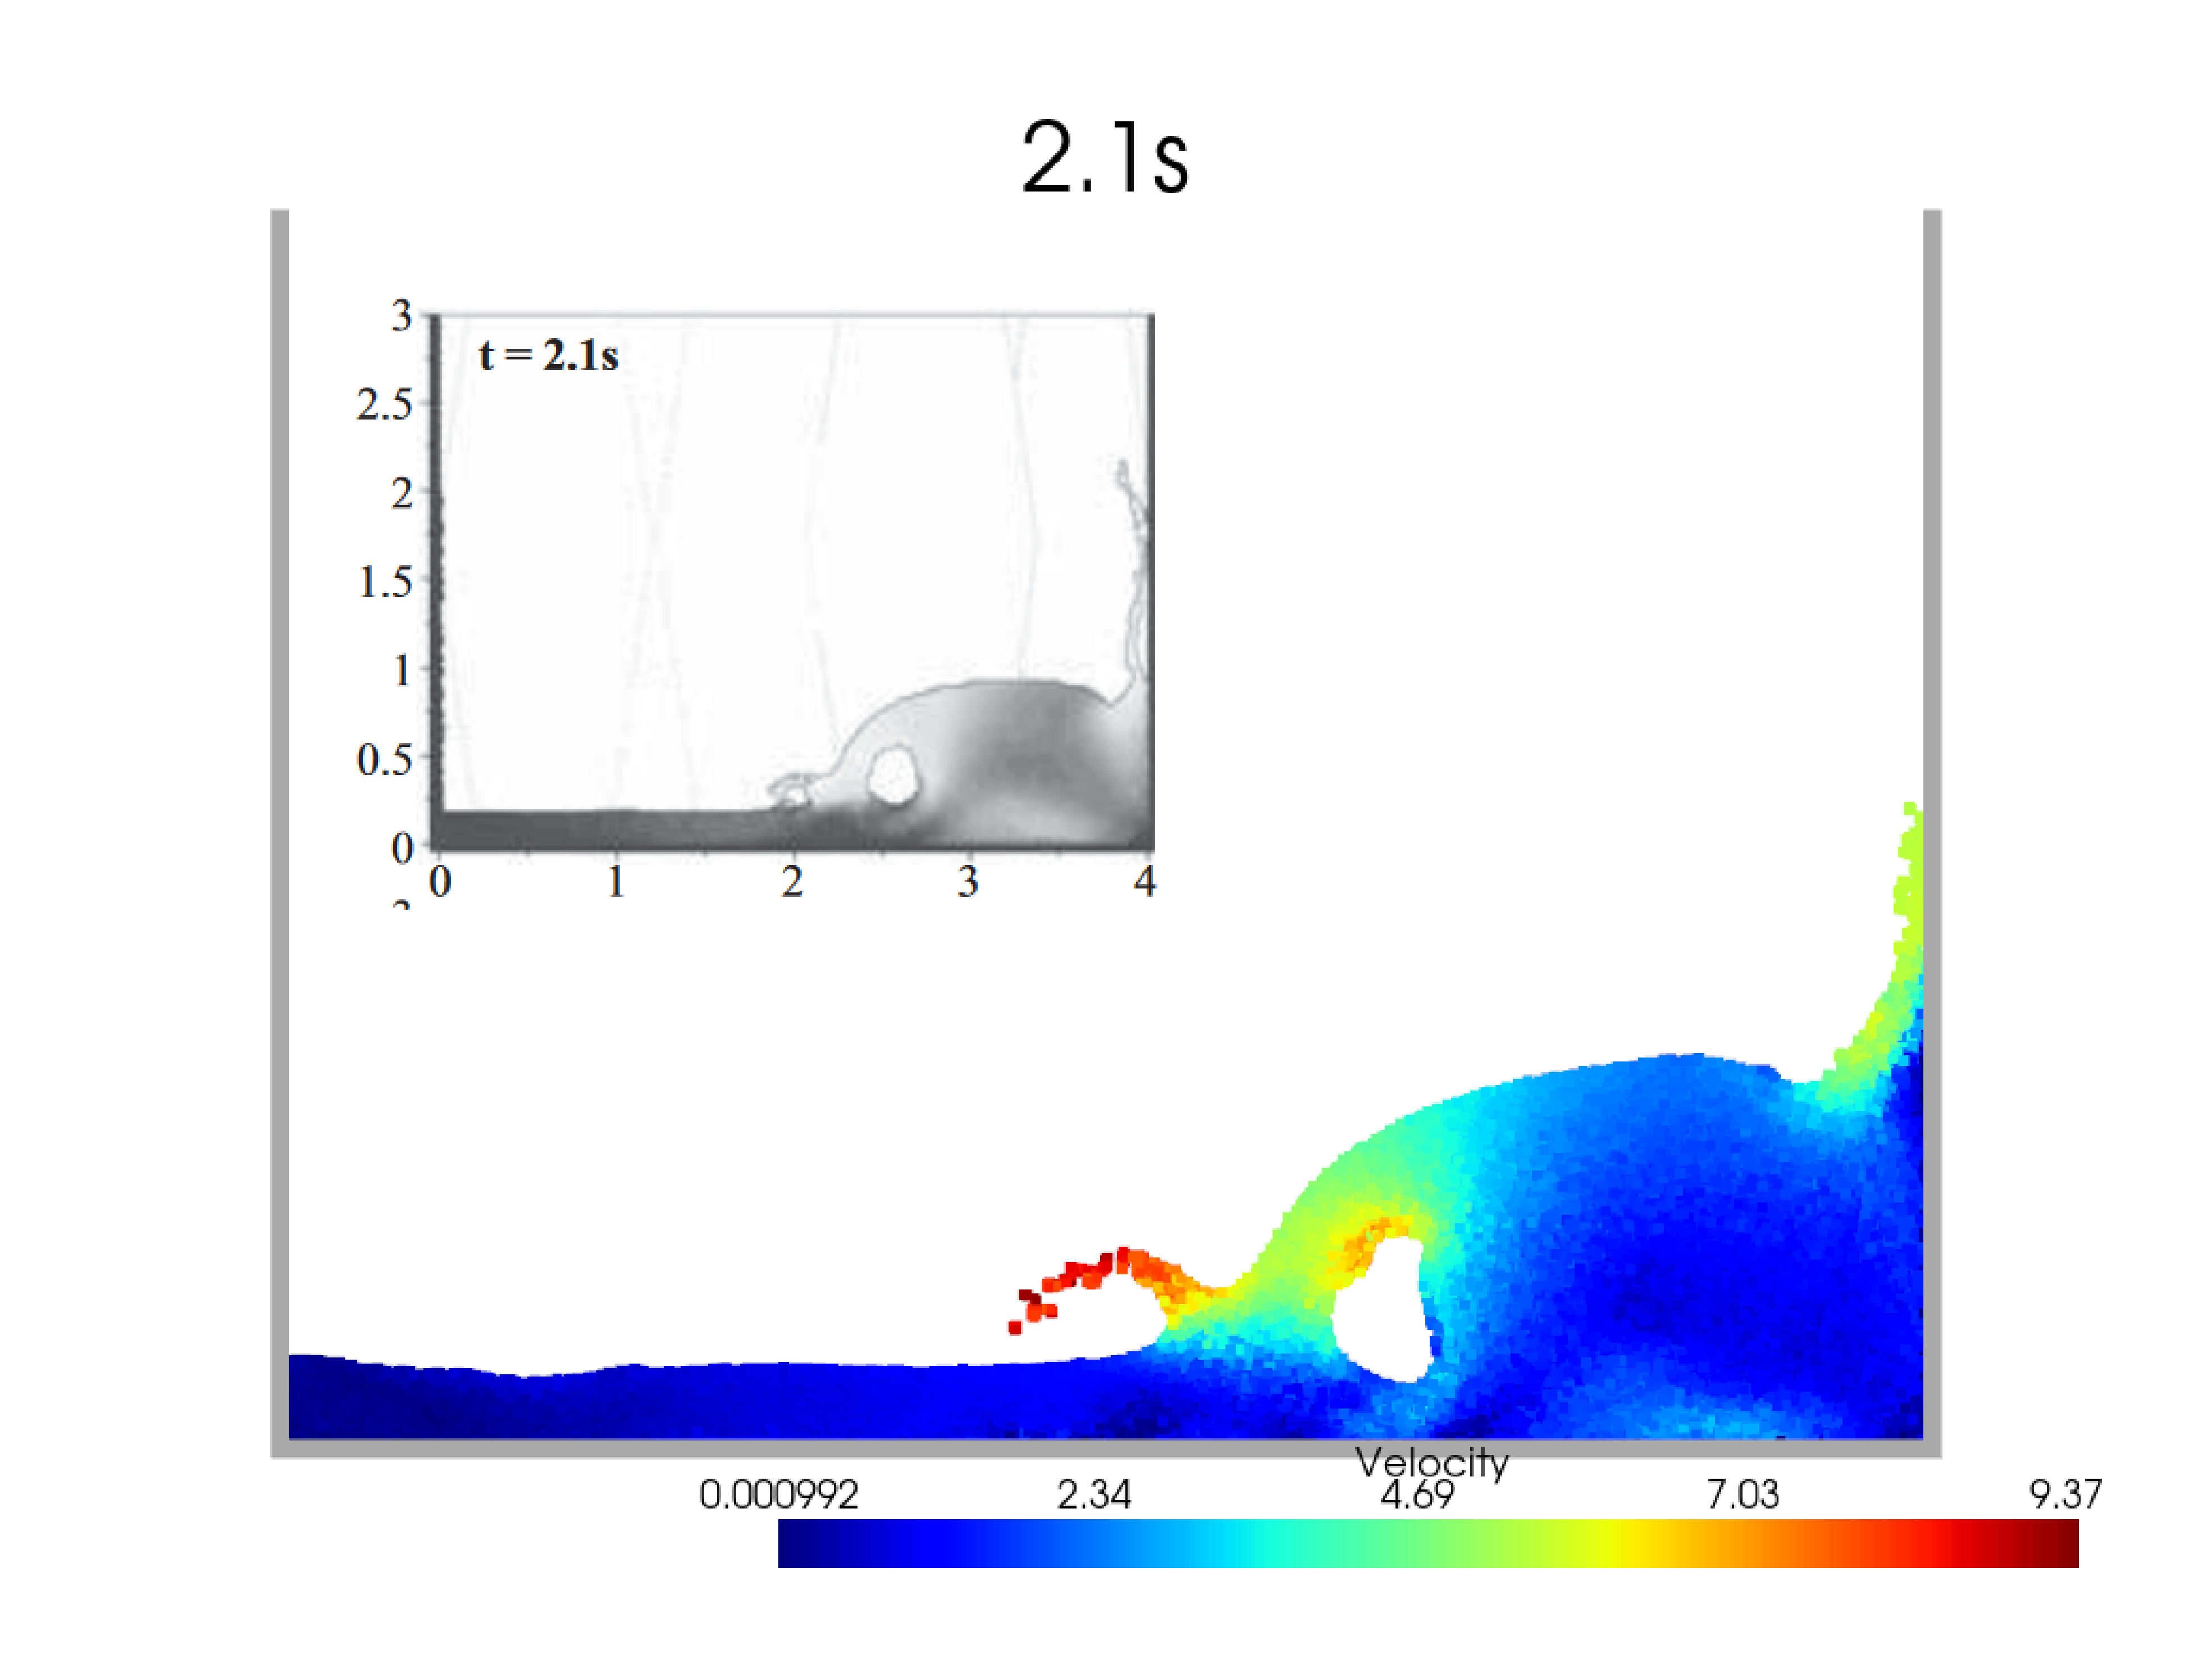
\includegraphics[width=0.47\textwidth]{images/CollapseDry/origin/collapse_dry21_combined.png}
        }
        \subfigure[壁面粒子垫高]{
            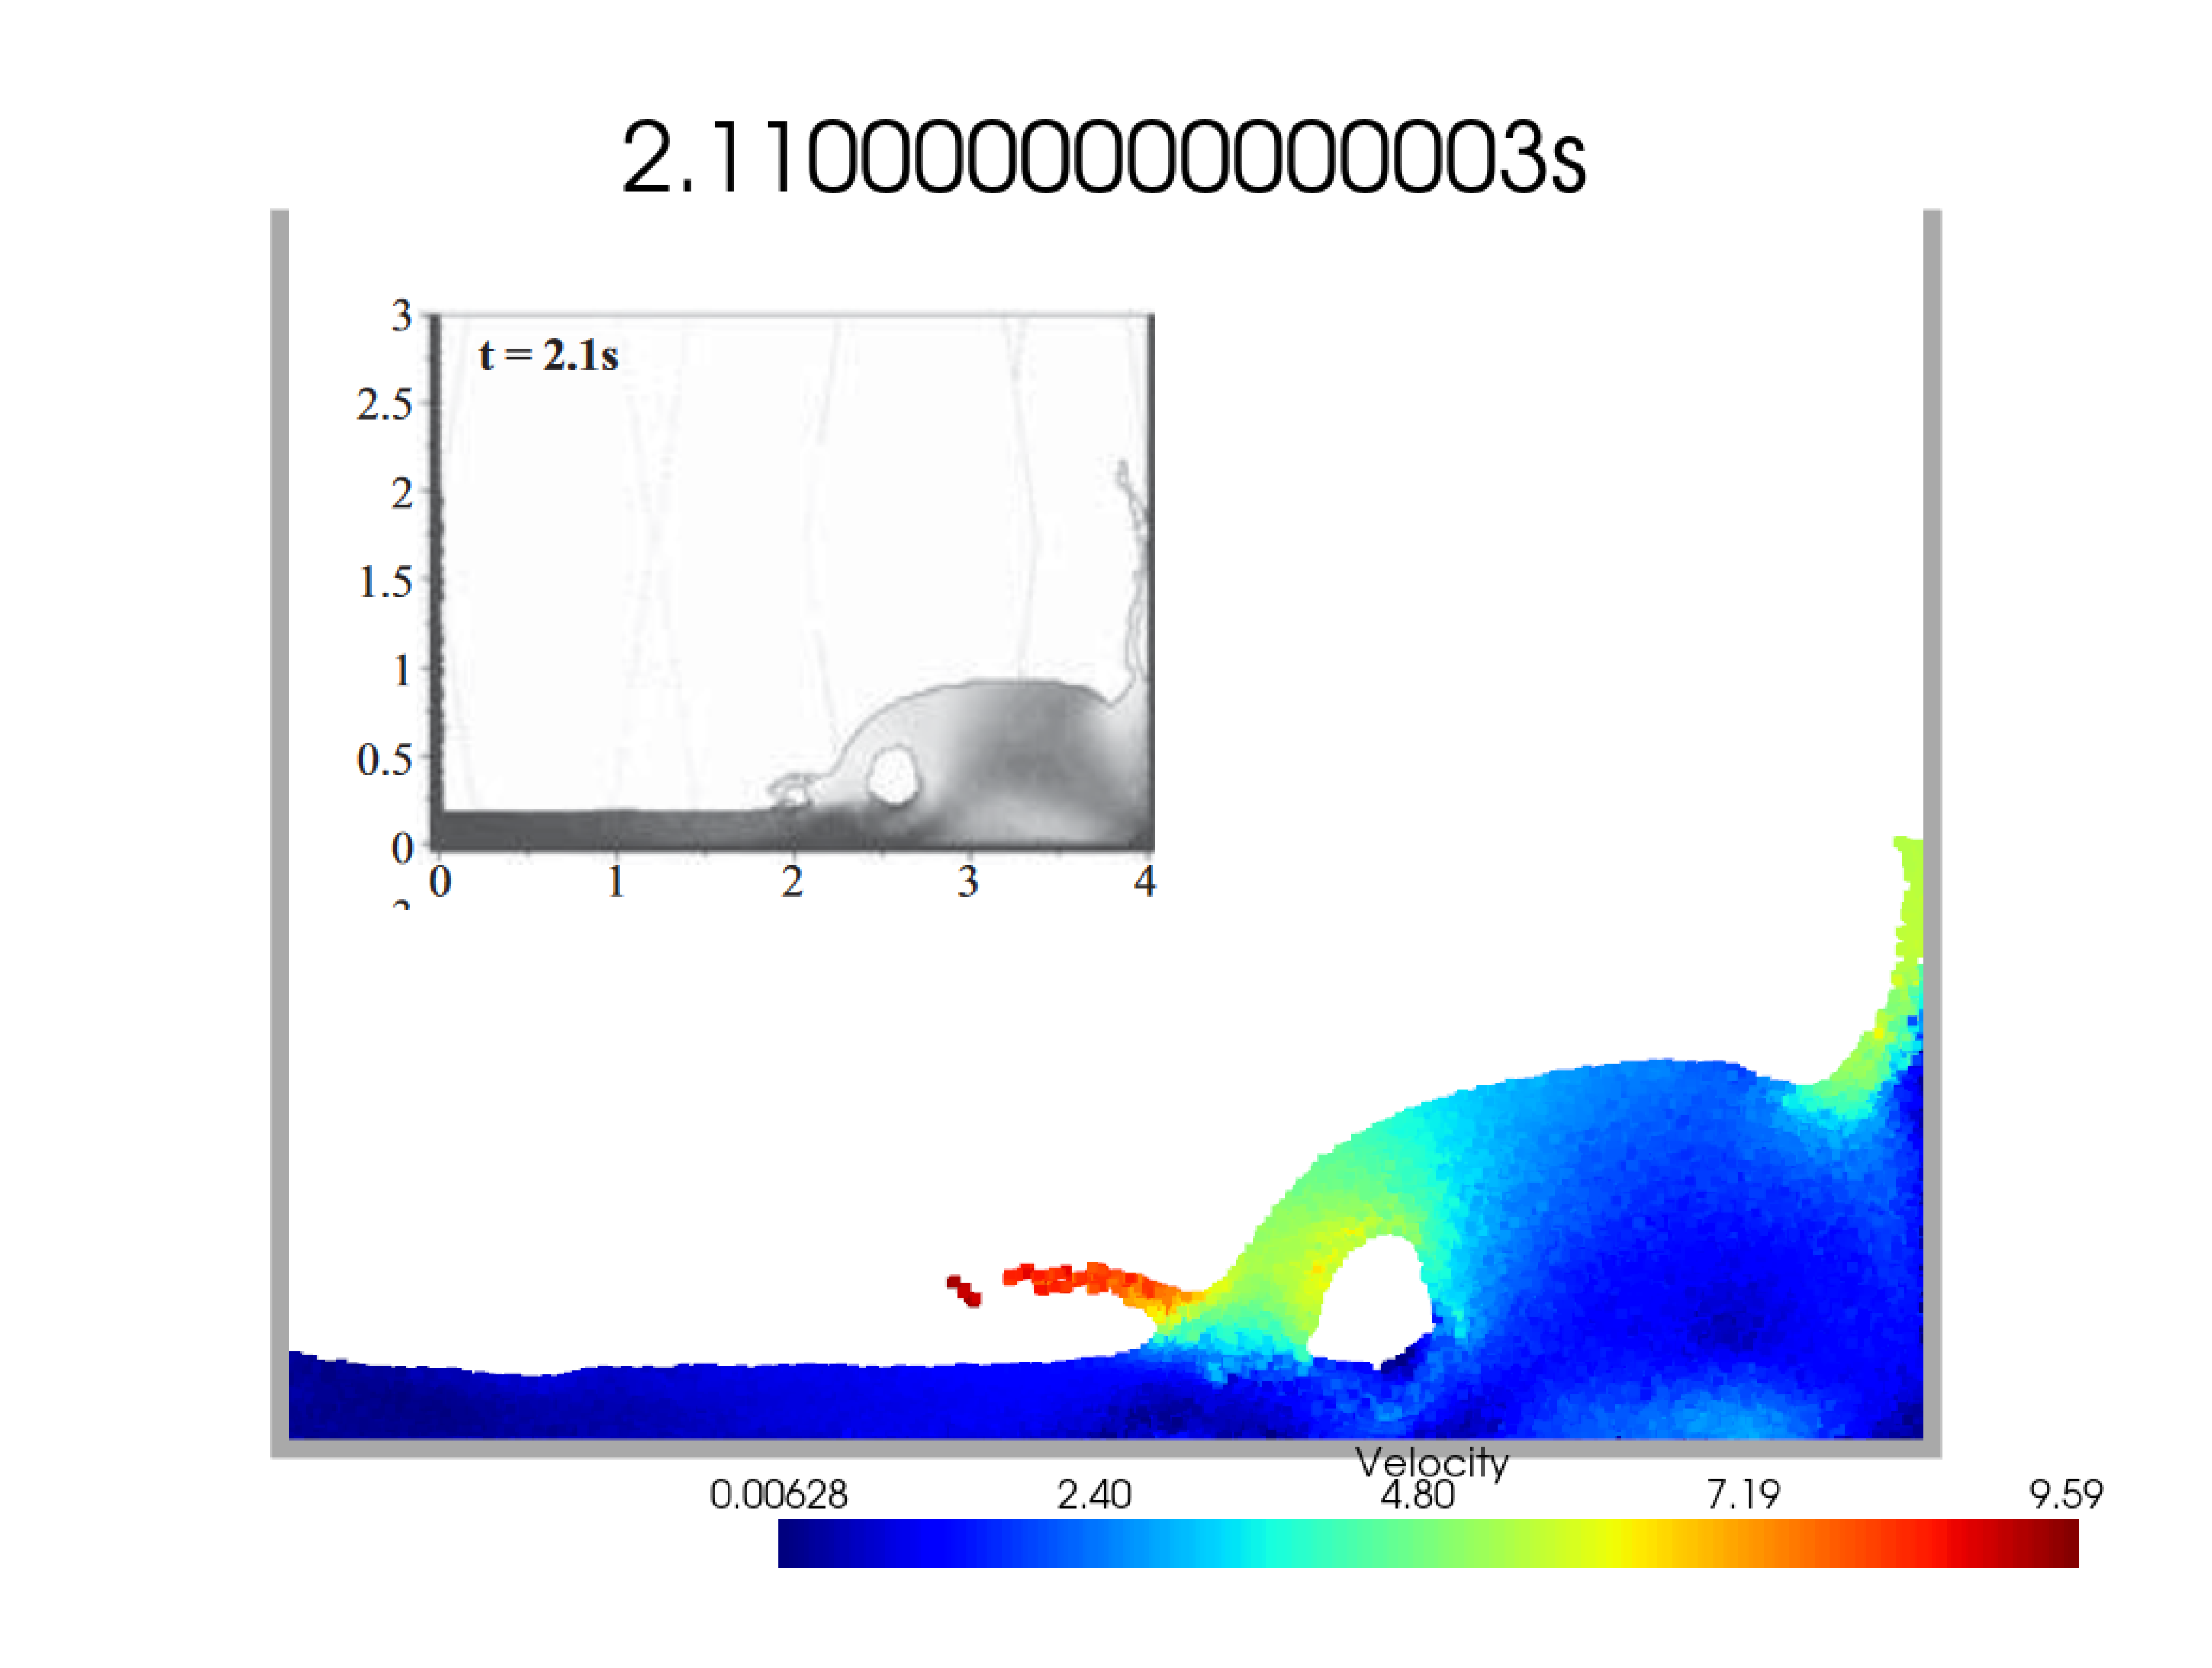
\includegraphics[width=0.47\textwidth]{images/CollapseDry/half/collapse_dry21_combined.png}
        }
    \end{figure}
\end{frame}

\begin{frame}
    \begin{figure}[H]
        \centering
        \subfigure[壁面粒子未垫高]{
            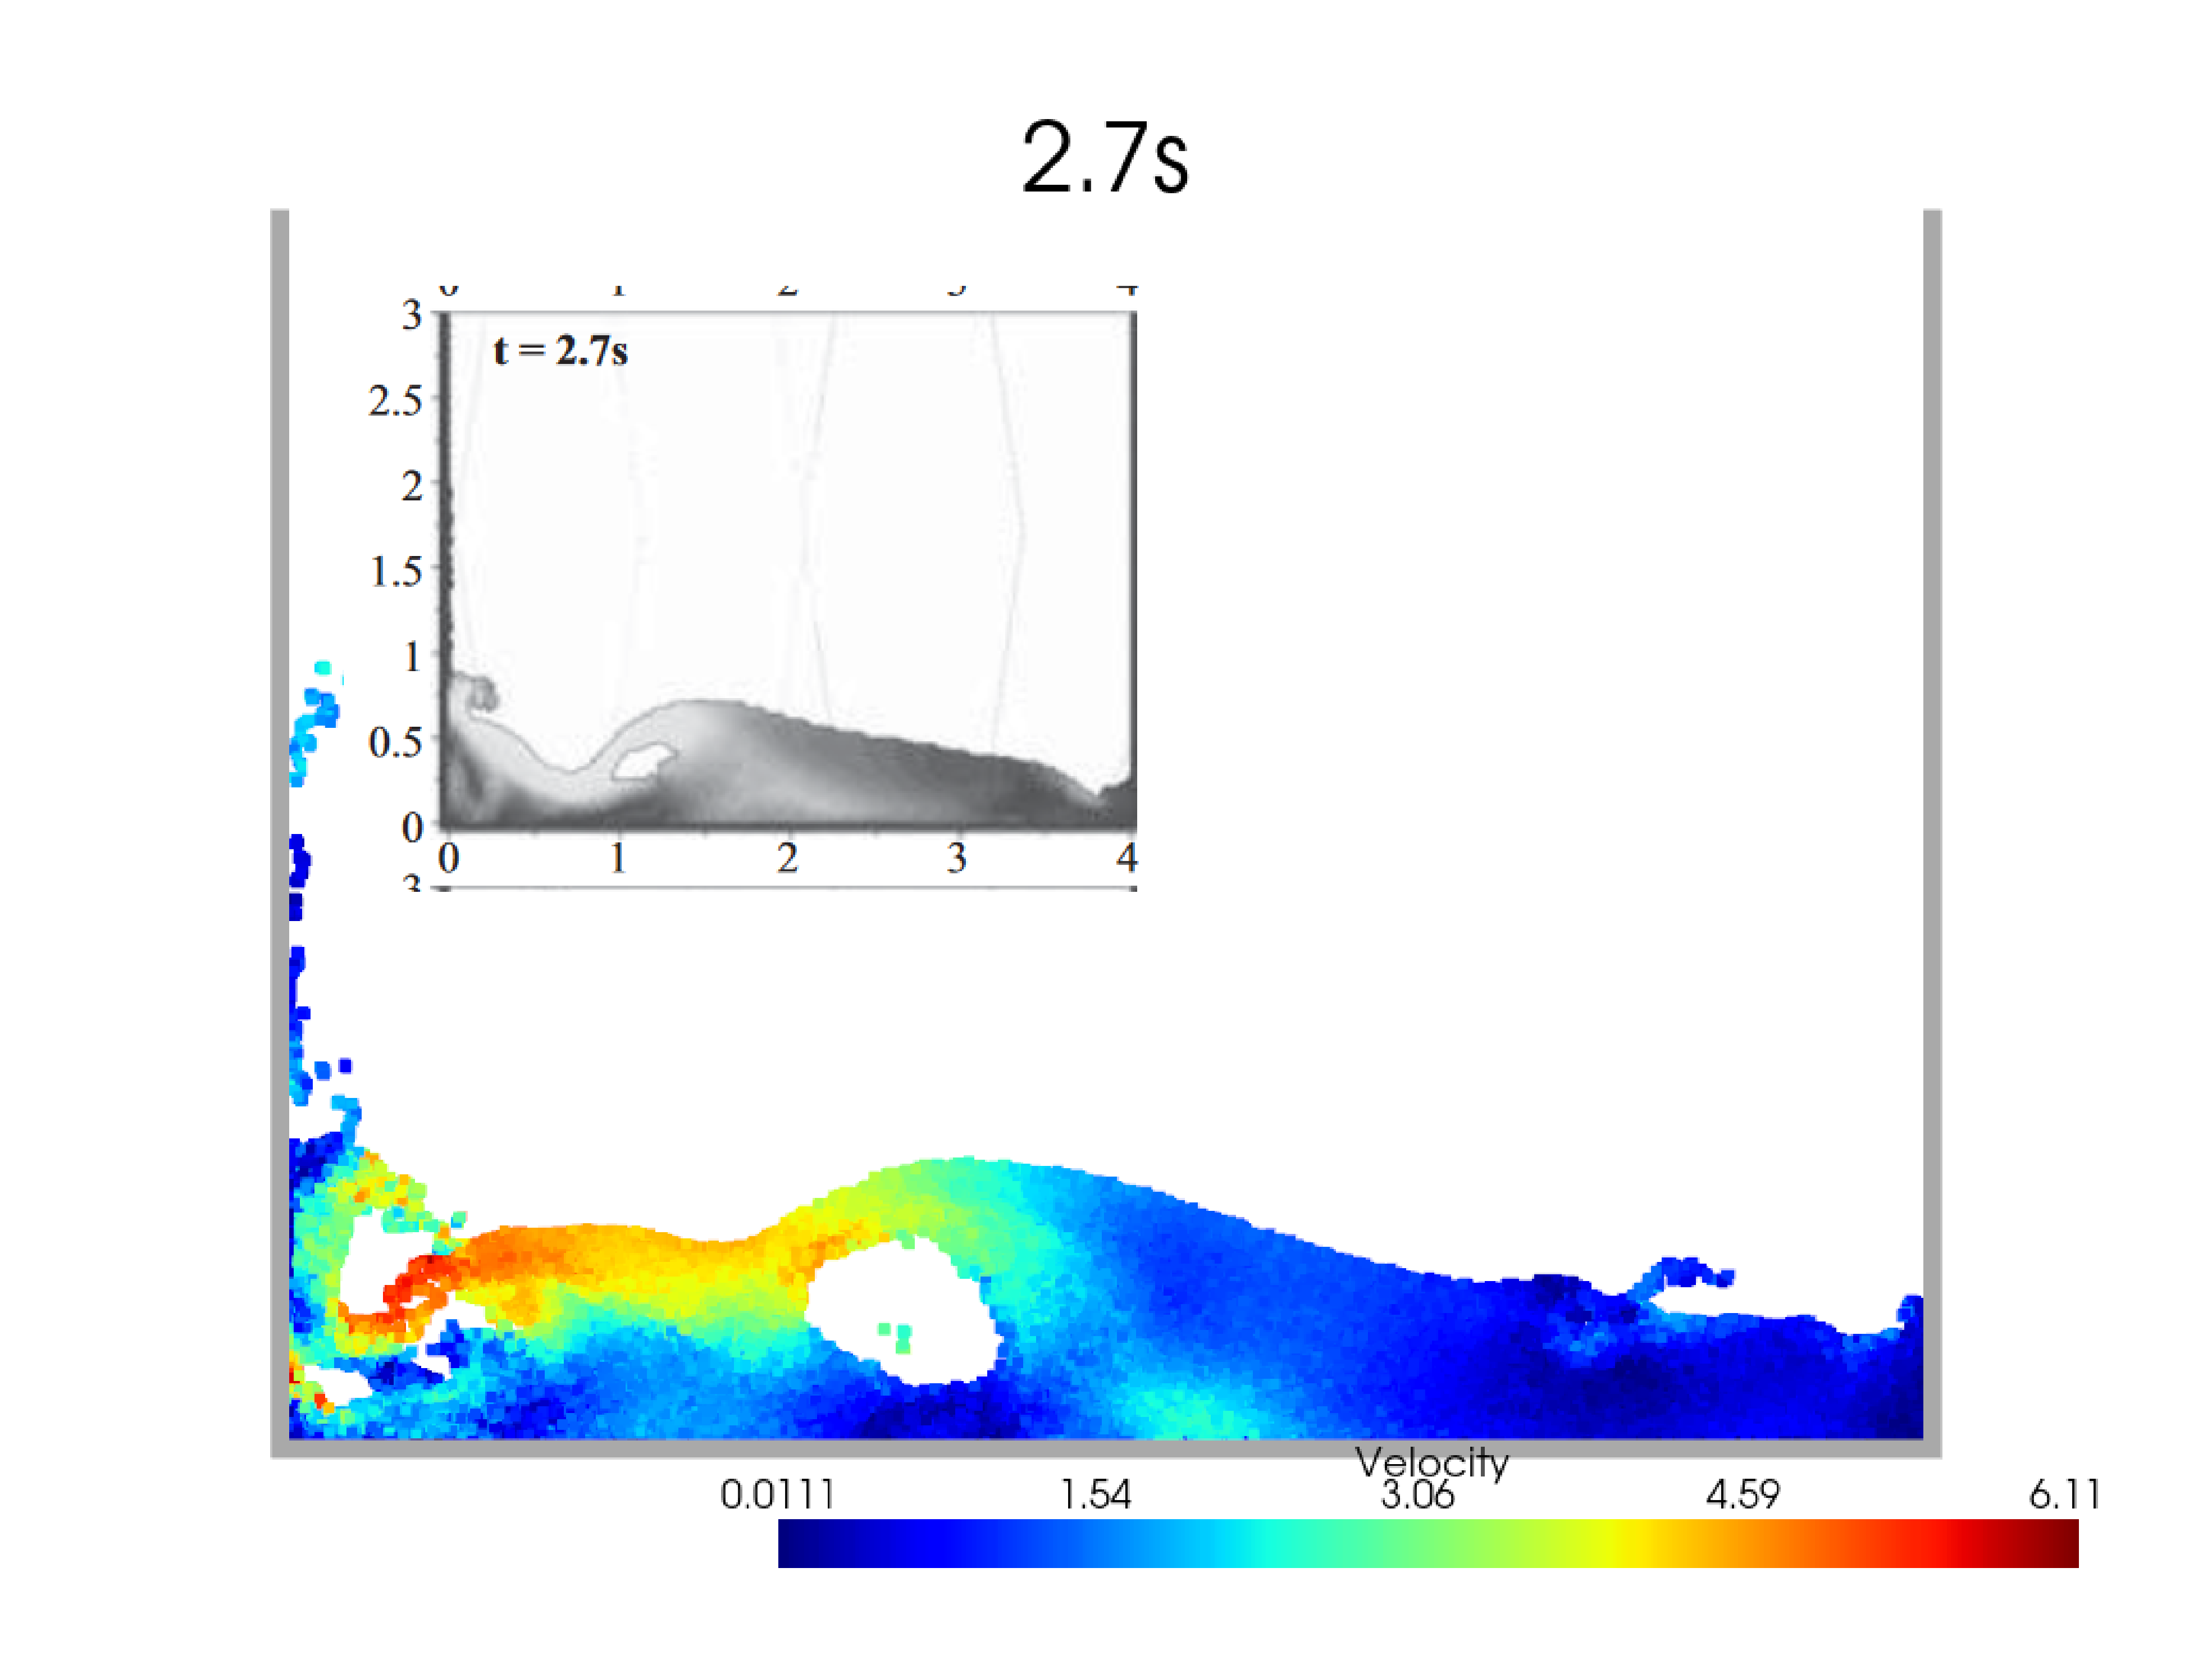
\includegraphics[width=0.47\textwidth]{images/CollapseDry/origin/collapse_dry27_combined.png}
        }
        \subfigure[壁面粒子垫高]{
            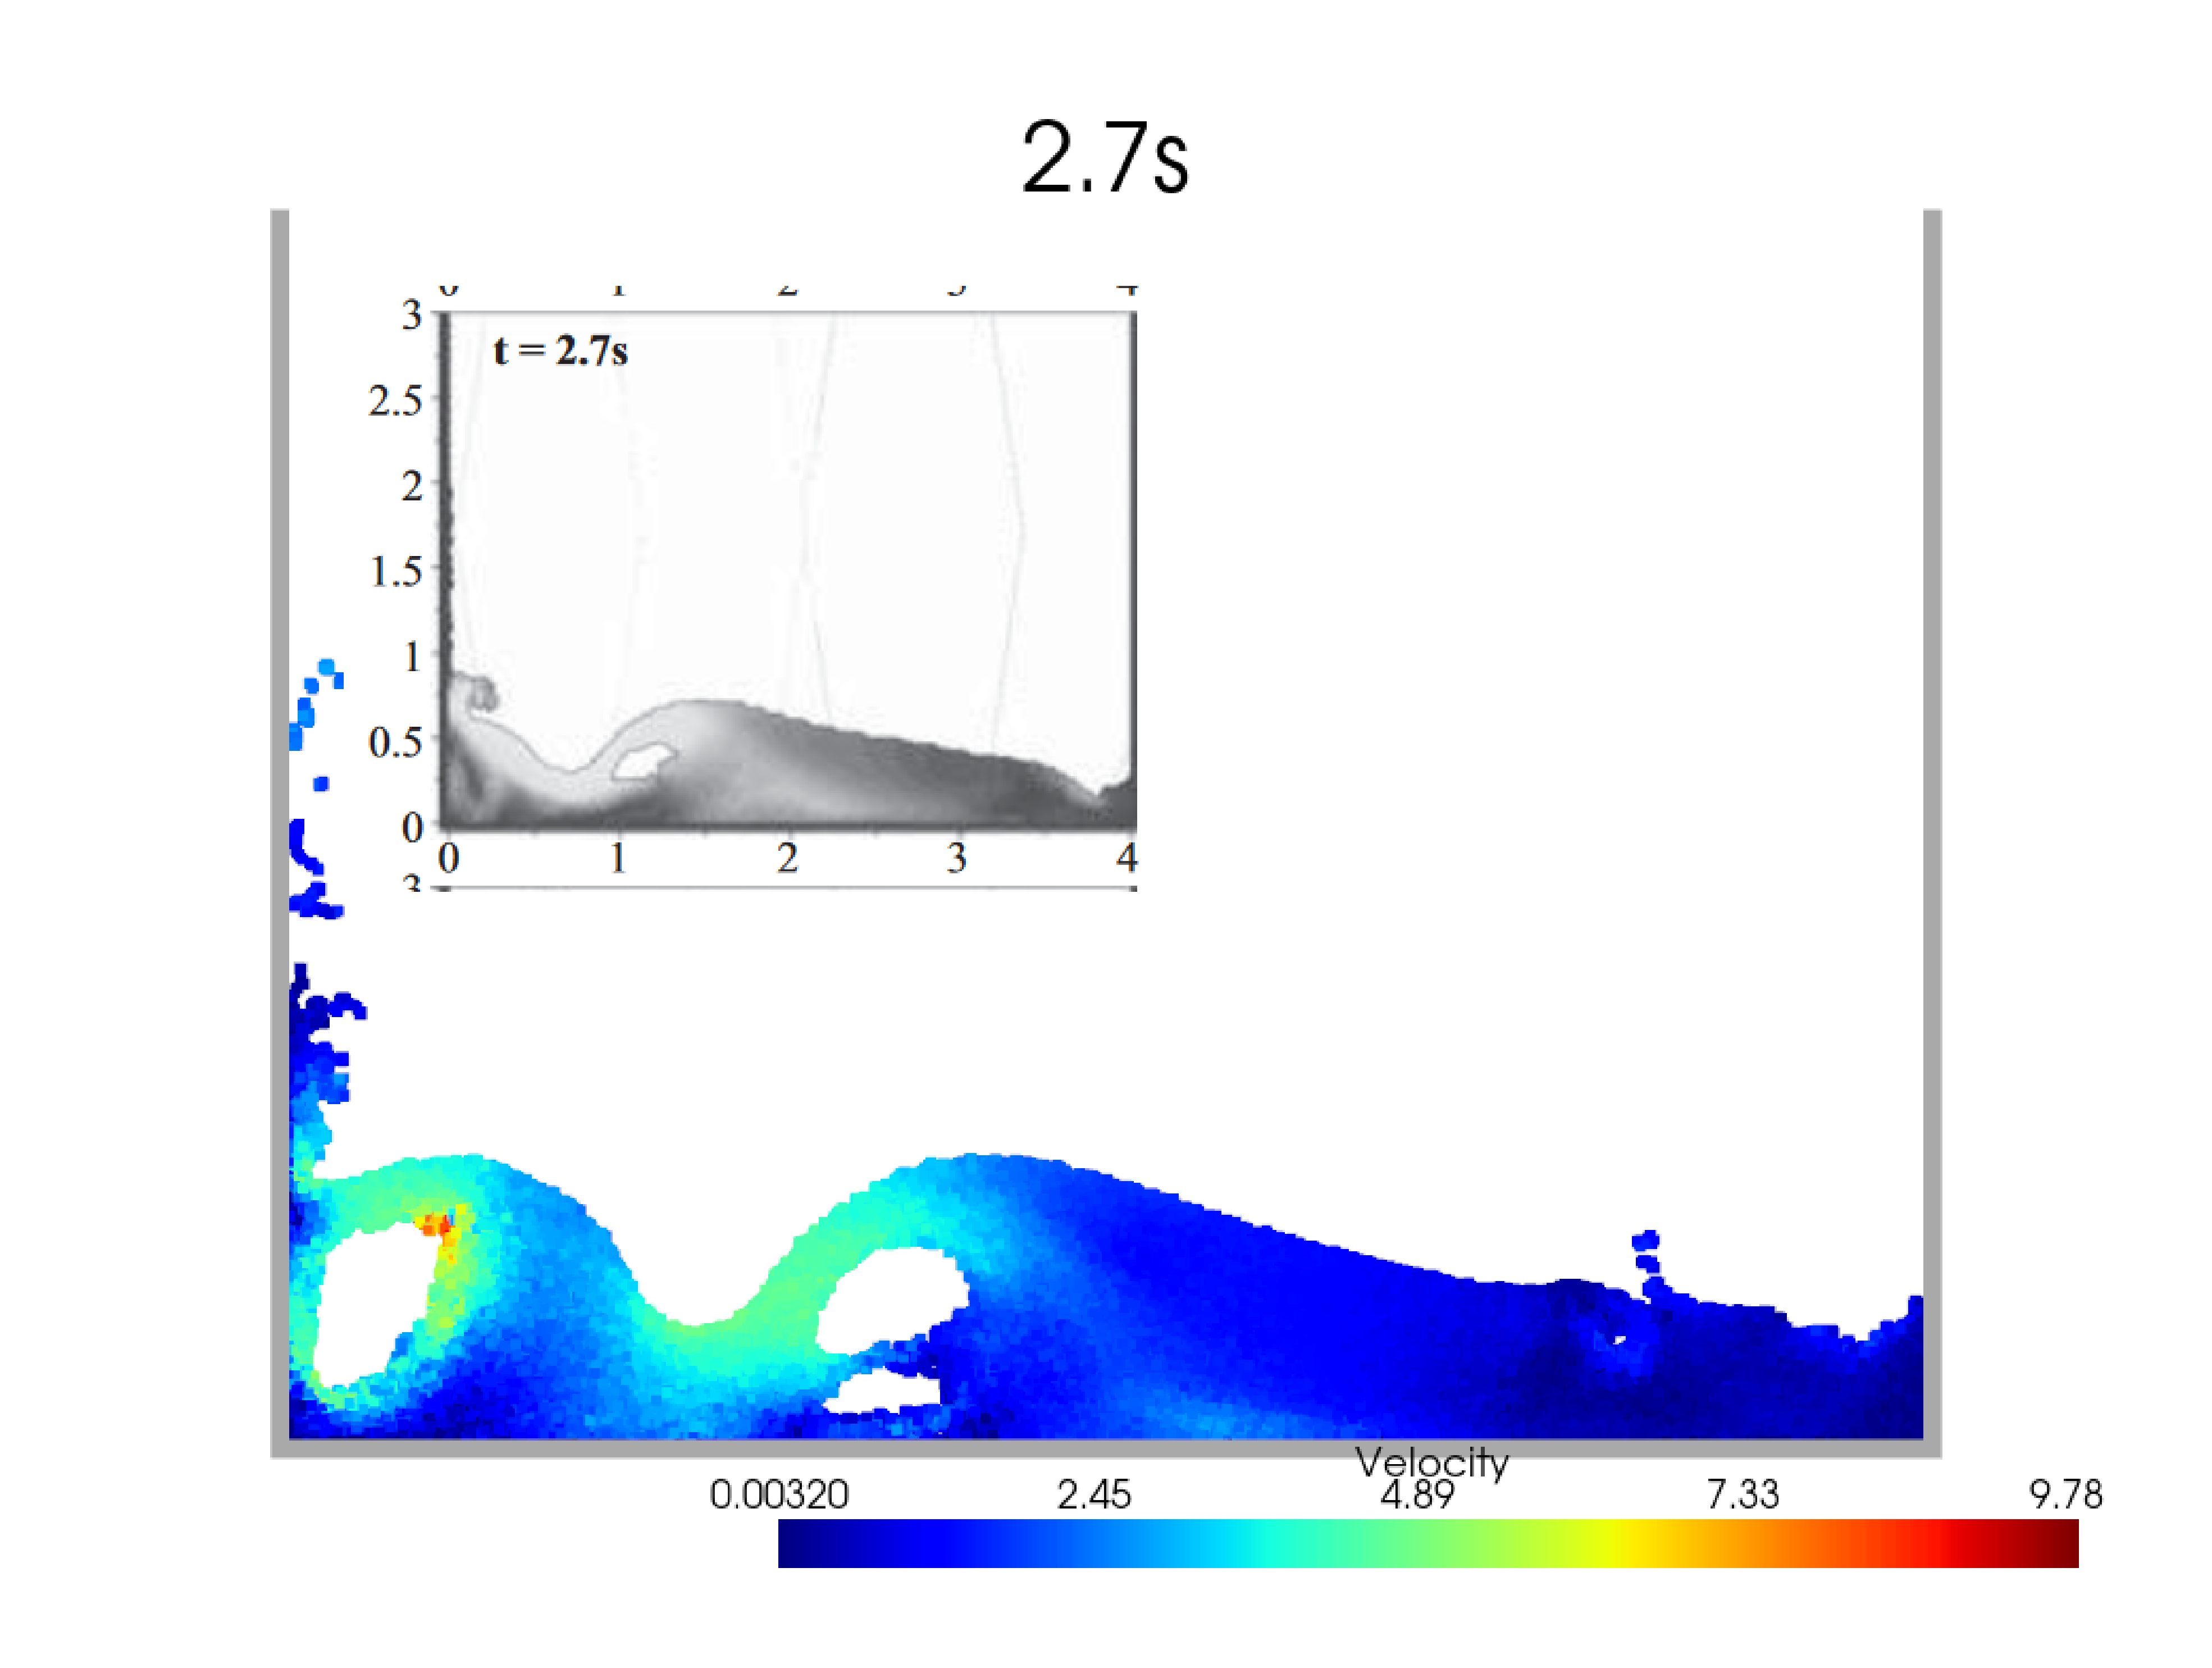
\includegraphics[width=0.47\textwidth]{images/CollapseDry/half/collapse_dry27_combined.png}
        }
    \end{figure}
\end{frame}

\begin{frame}
    \begin{figure}[H]
        \centering
        \subfigure[壁面粒子未垫高]{
            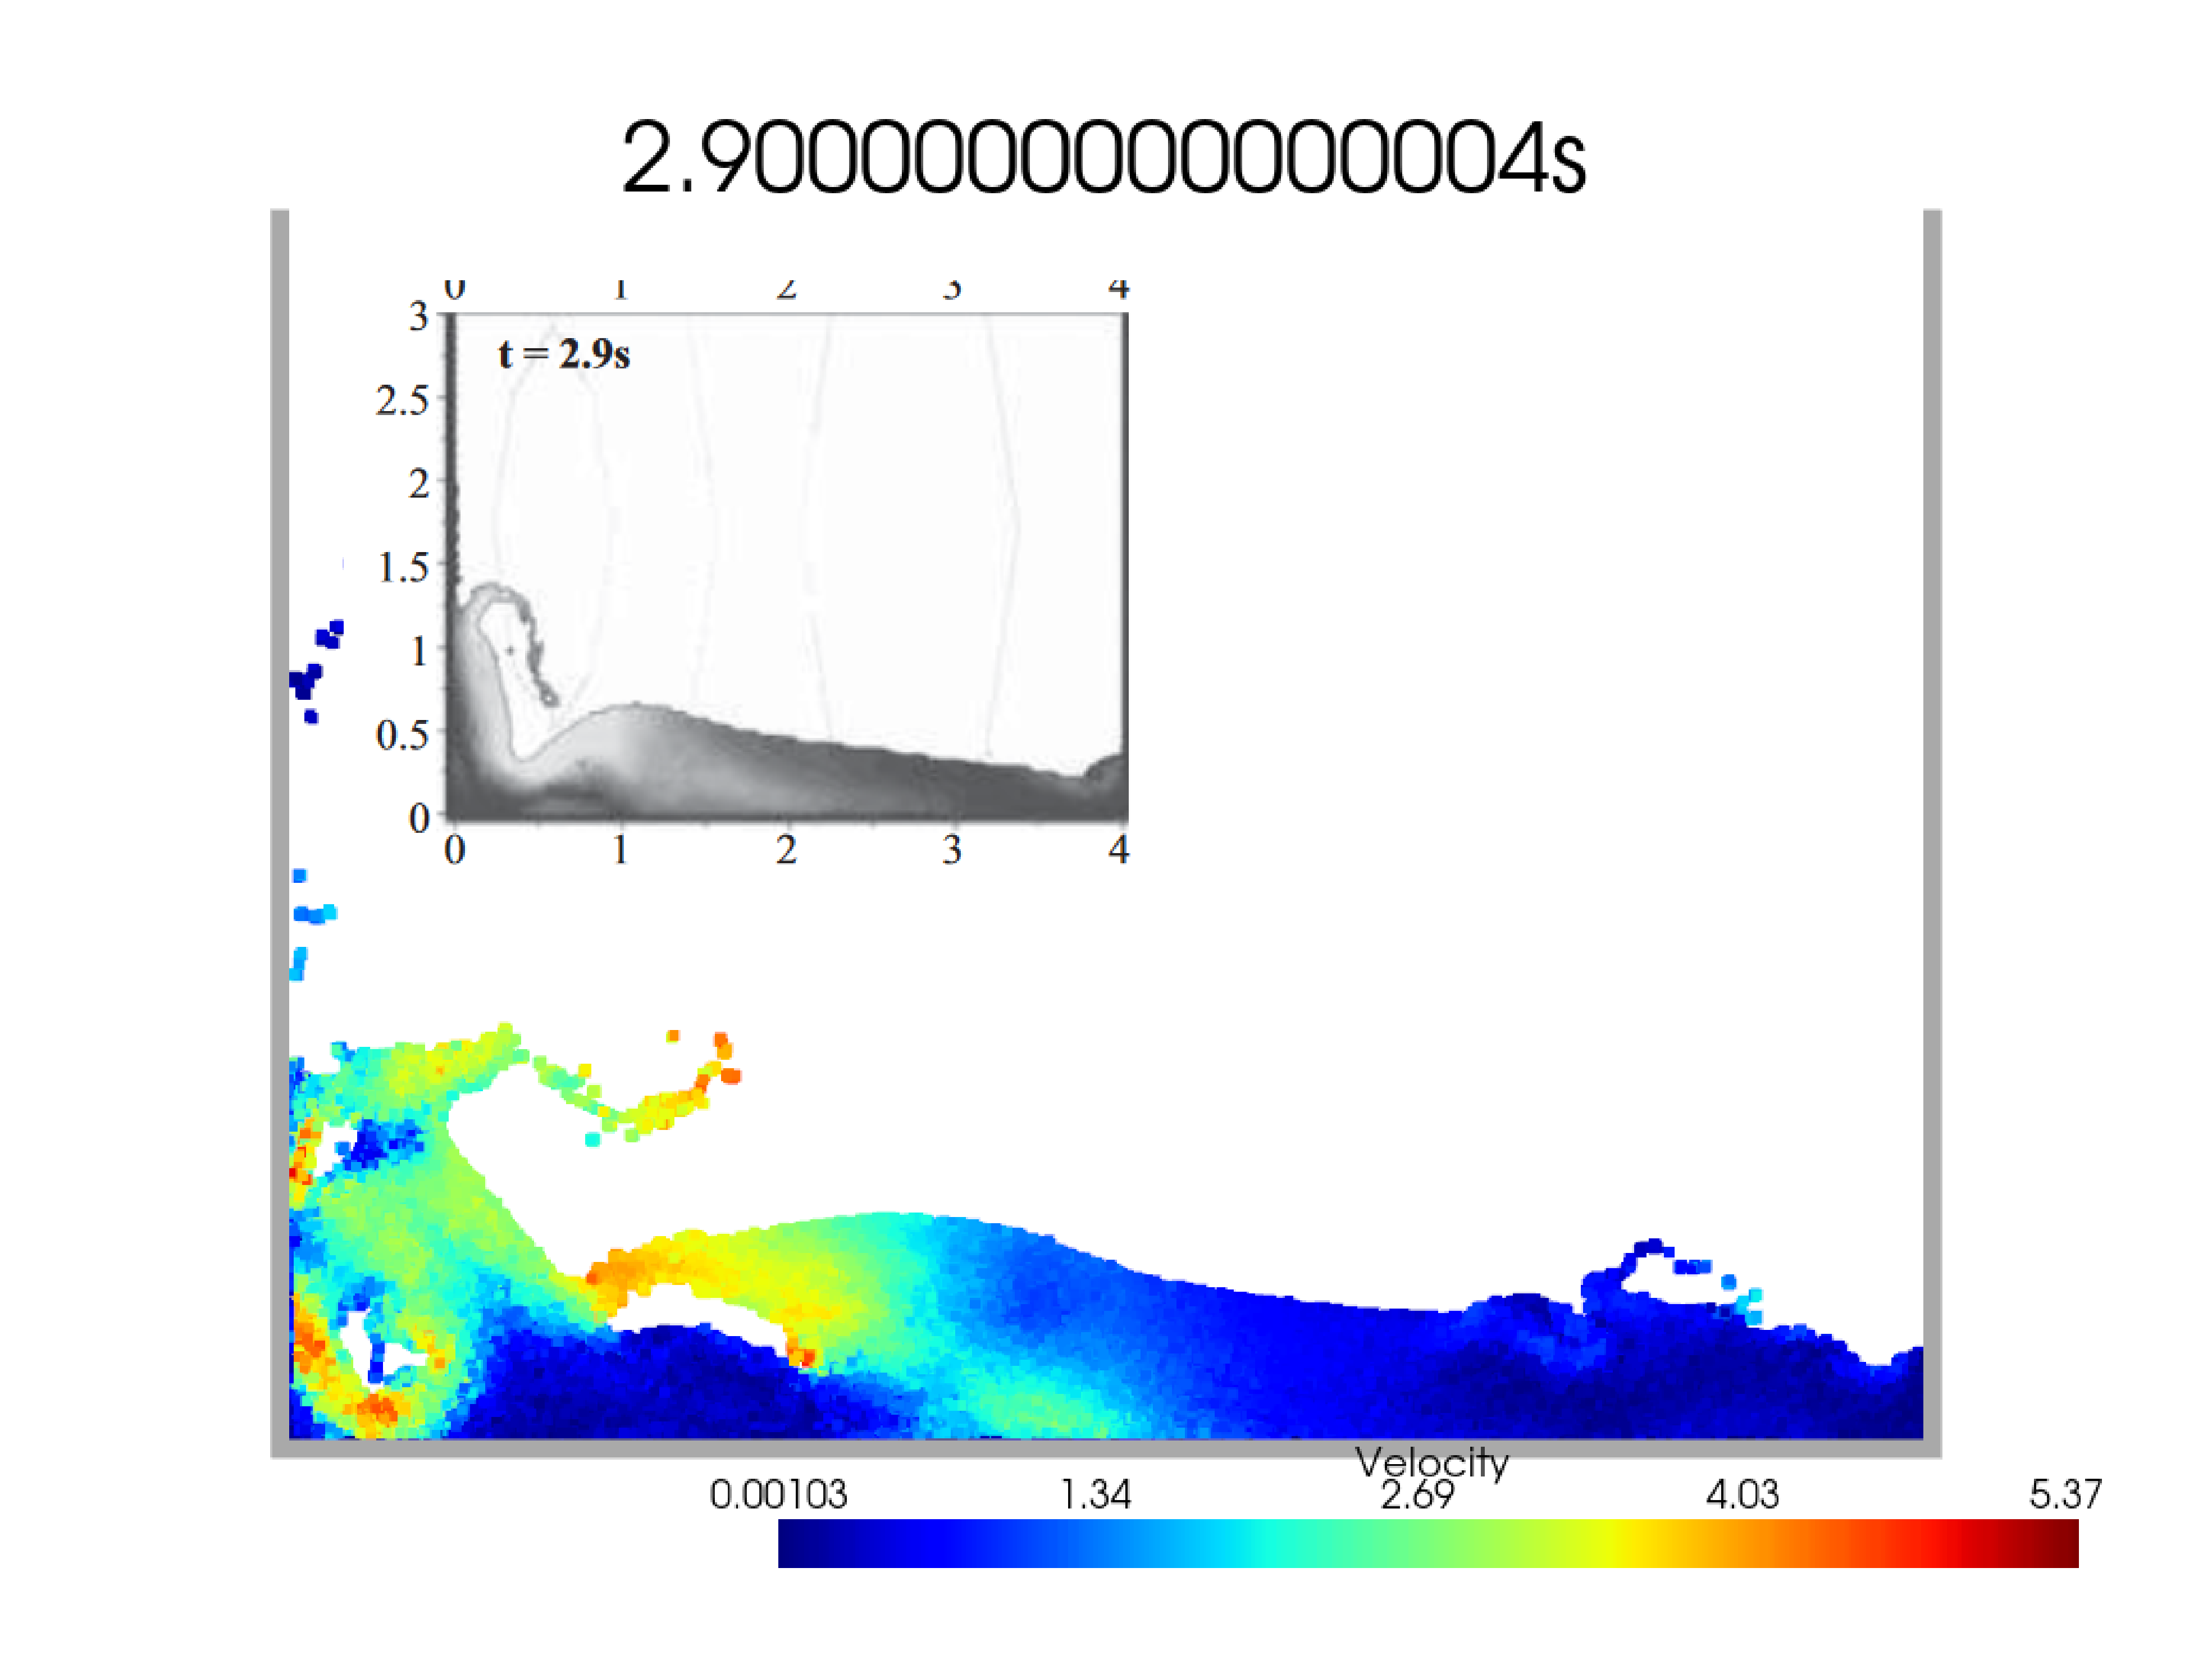
\includegraphics[width=0.47\textwidth]{images/CollapseDry/origin/collapse_dry29_combined.png}
        }
        \subfigure[壁面粒子垫高]{
            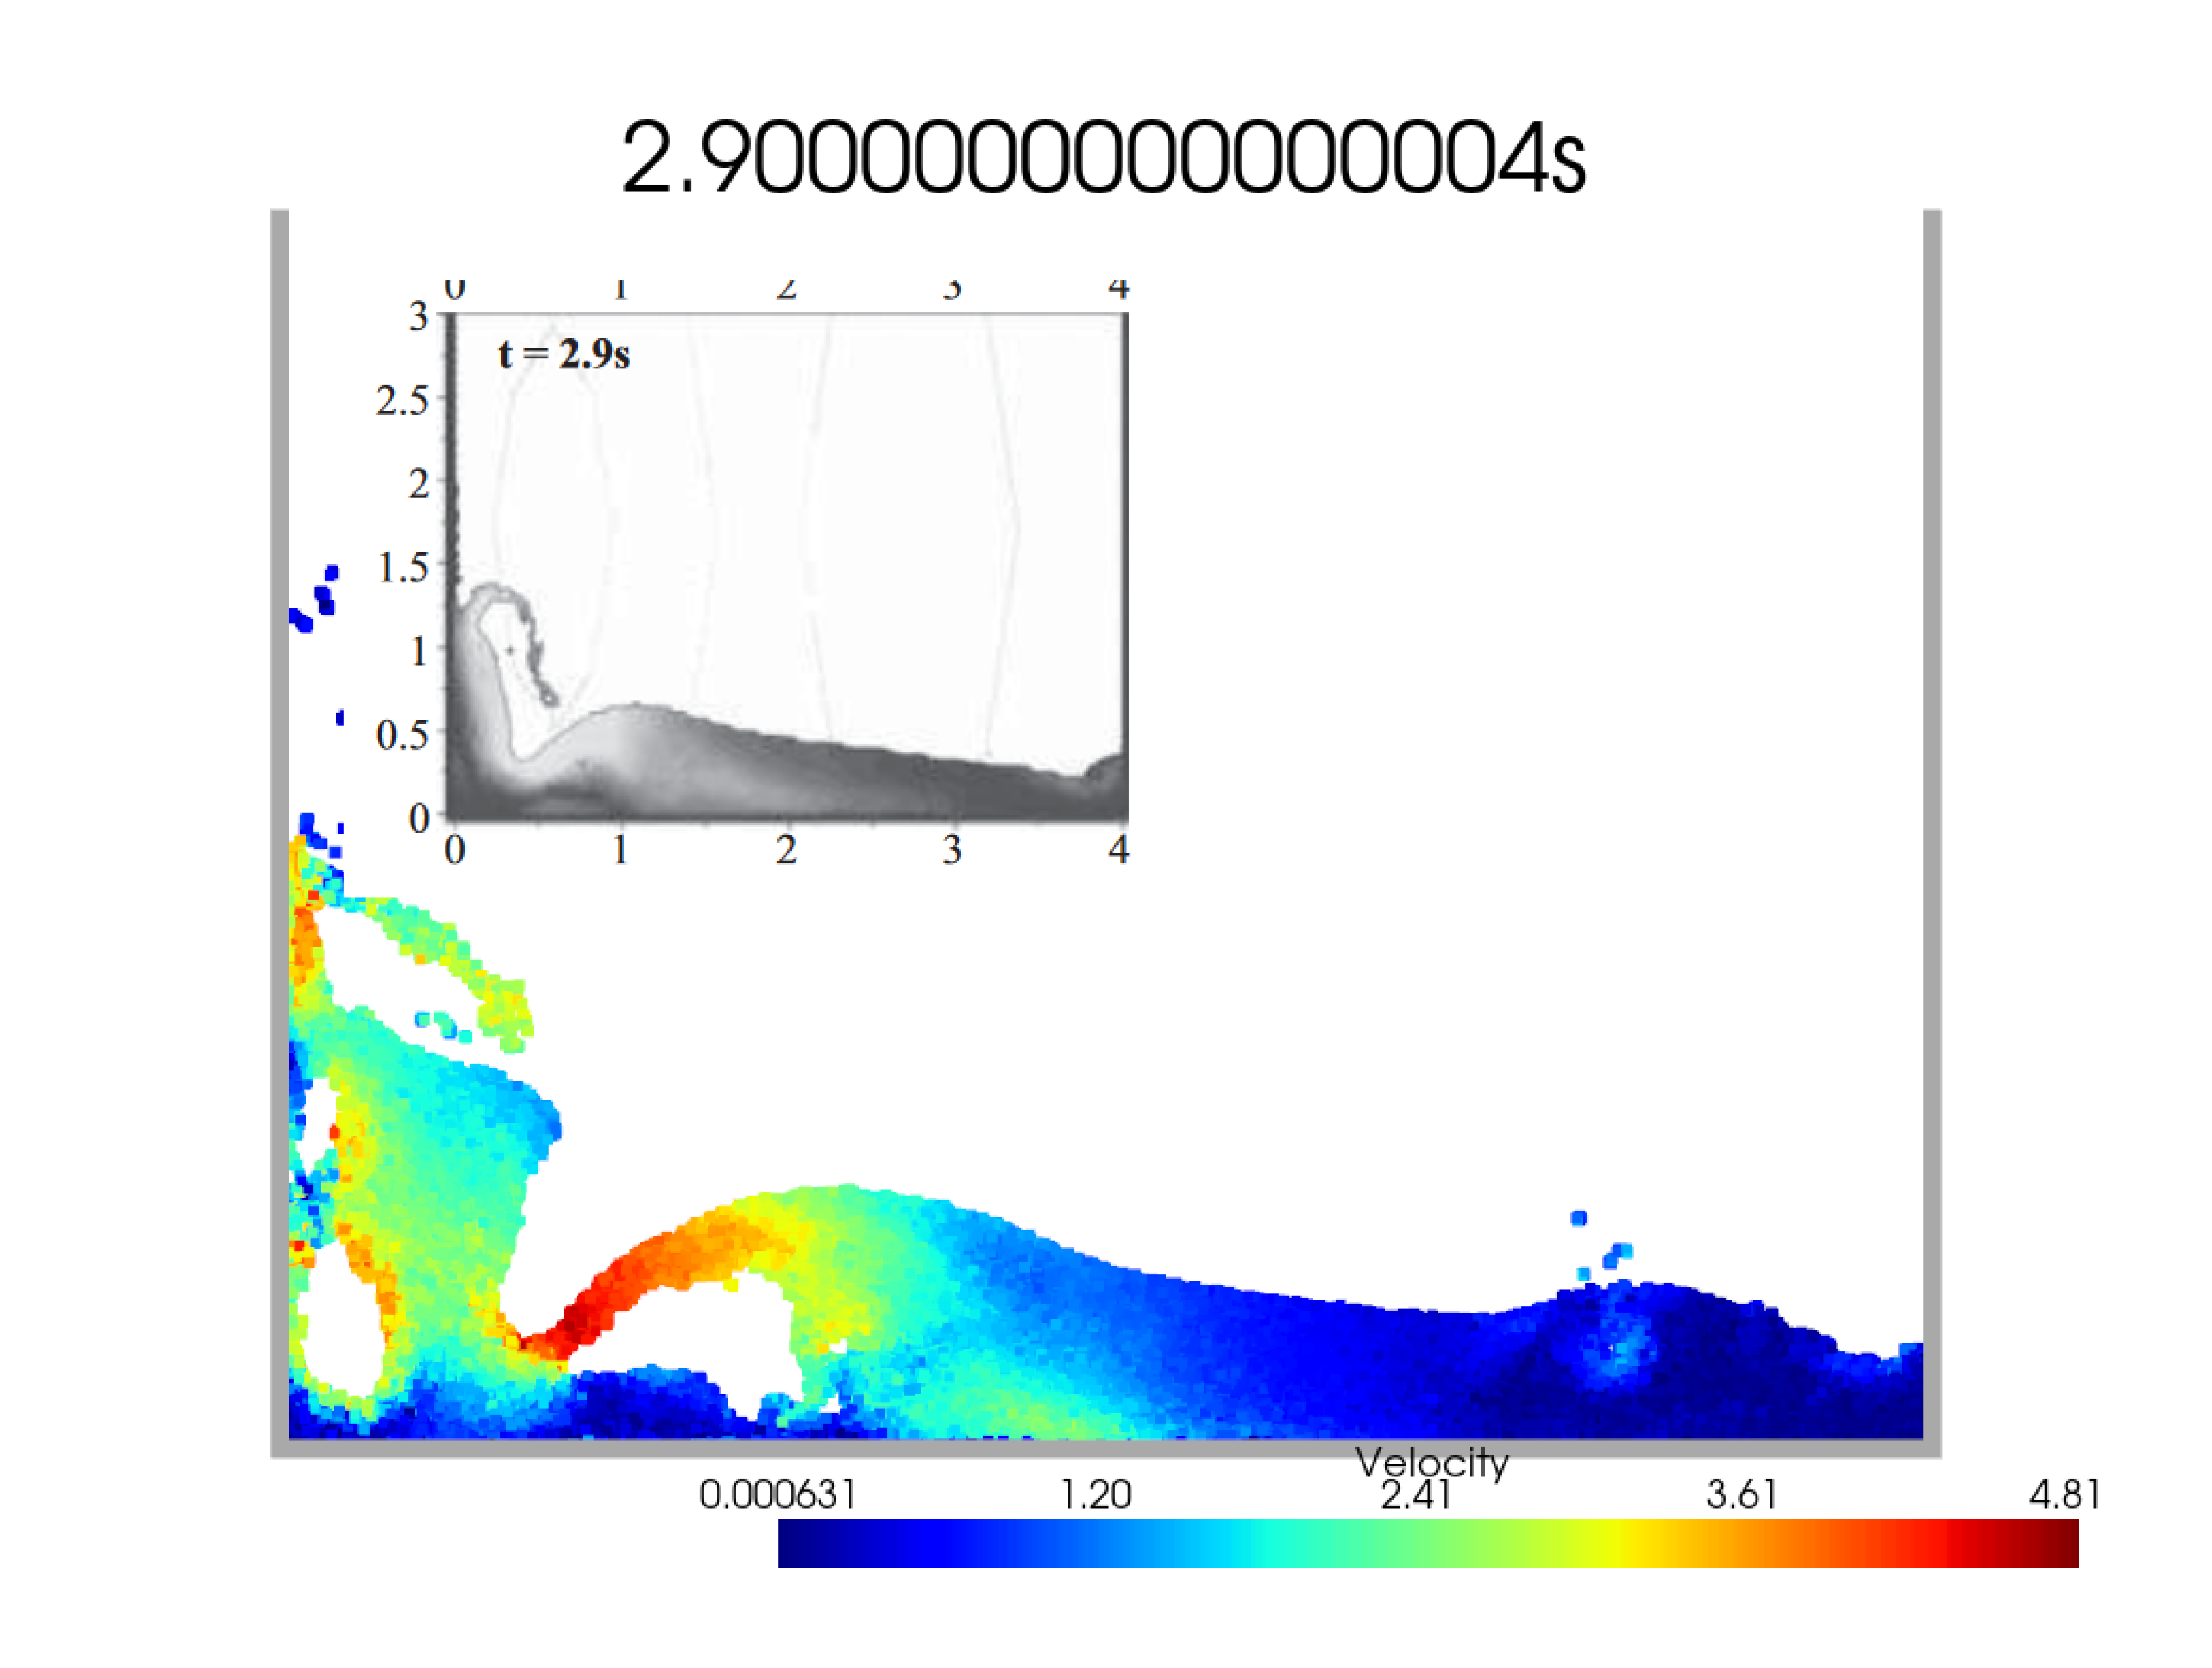
\includegraphics[width=0.47\textwidth]{images/CollapseDry/half/collapse_dry29_combined.png}
        }
    \end{figure}
\end{frame}

\begin{frame}
    在这个算例中,
    标准算例提供的图片并没有明确指出壁面是怎么处理的(因为书中都是讲完三四种壁面方法,
    最后才提供算例的结果),
    但并不在算例中指出采用了什么壁面条件。
    算例从液体回注开始,和标准算例差别比较大,
    但在垮塌过程中曲线对比能对上。
    \begin{figure}[H]
        \centering
        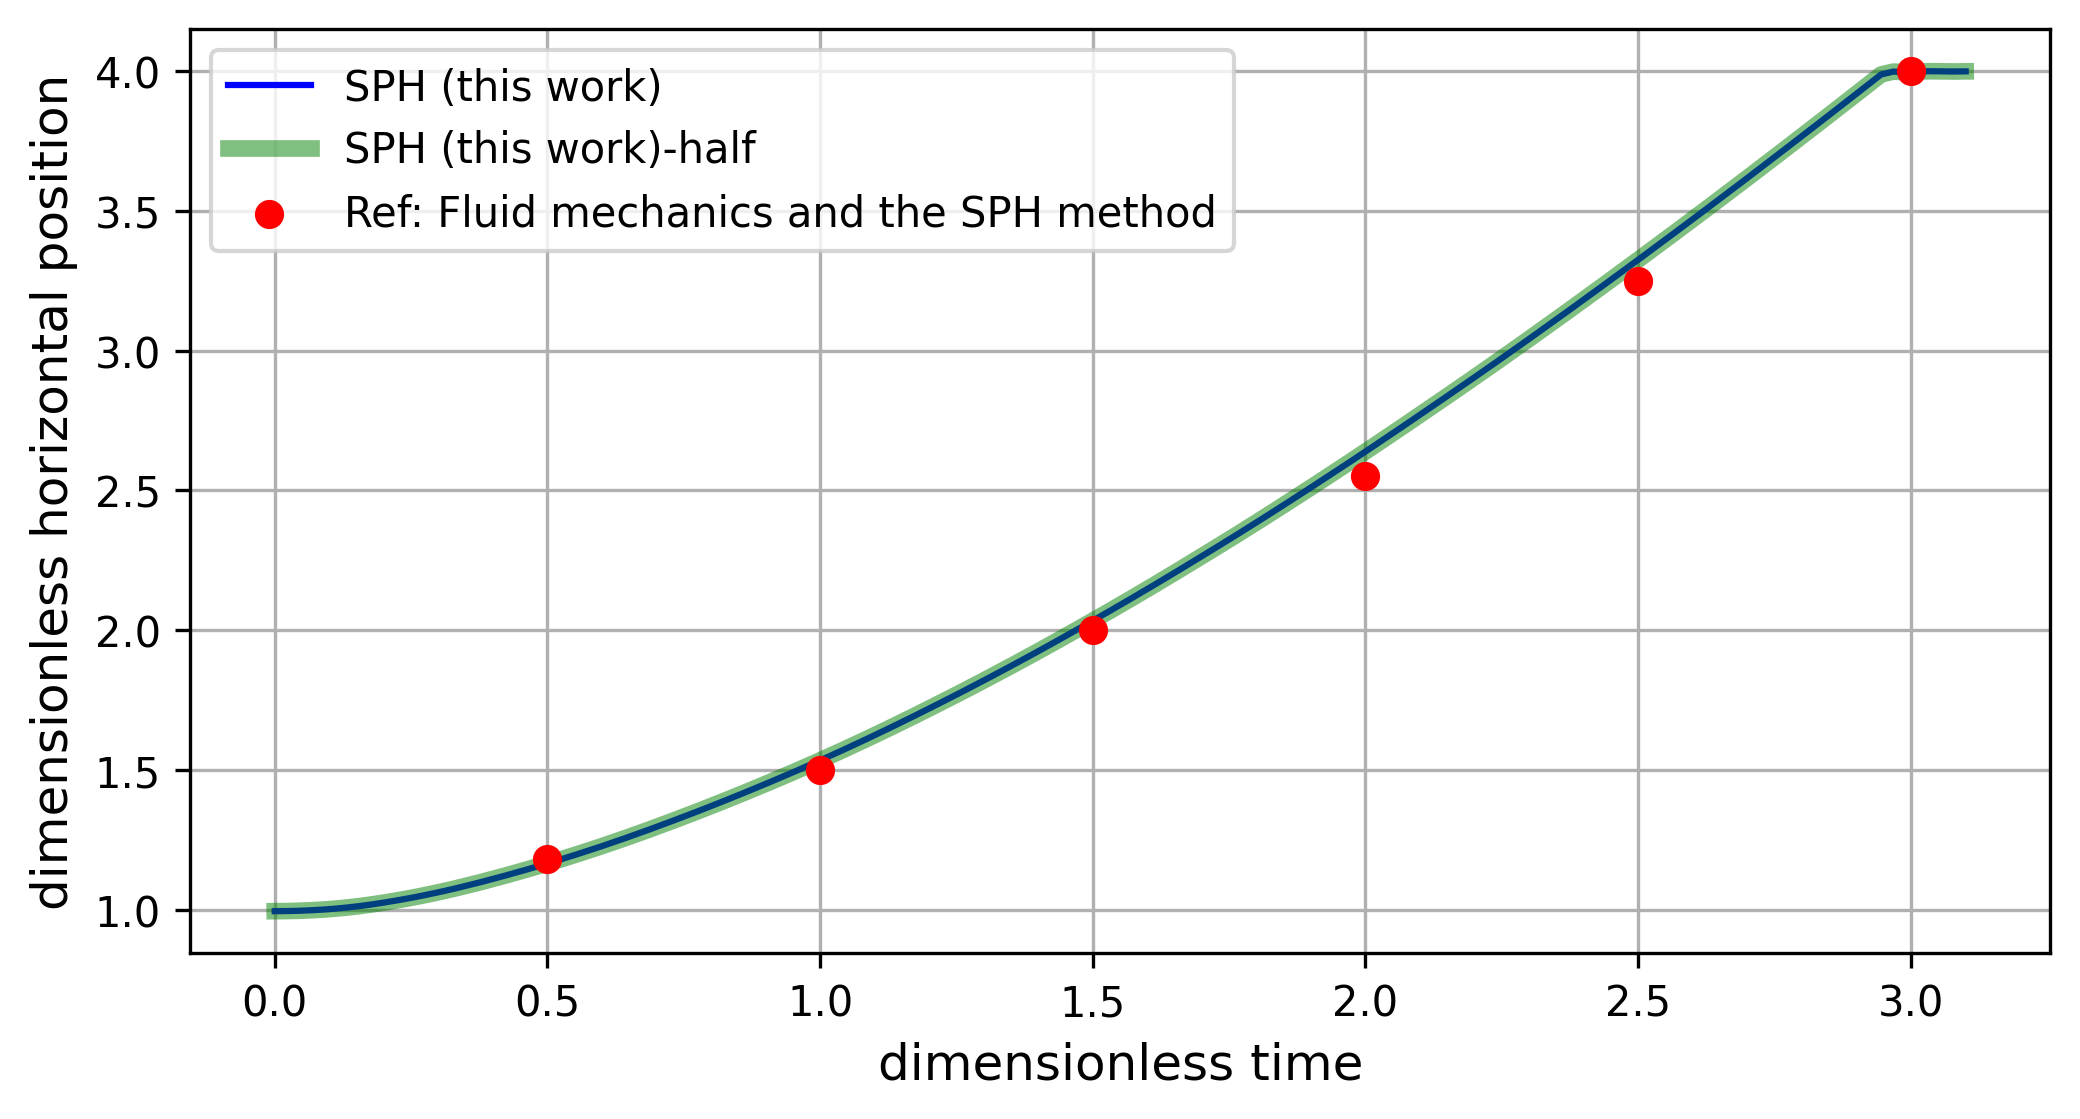
\includegraphics[width=\textwidth]{images/CollapseDry/horizontal_position.png}
    \end{figure}
\end{frame}

\begin{frame}
    \begin{figure}[H]
        \centering
        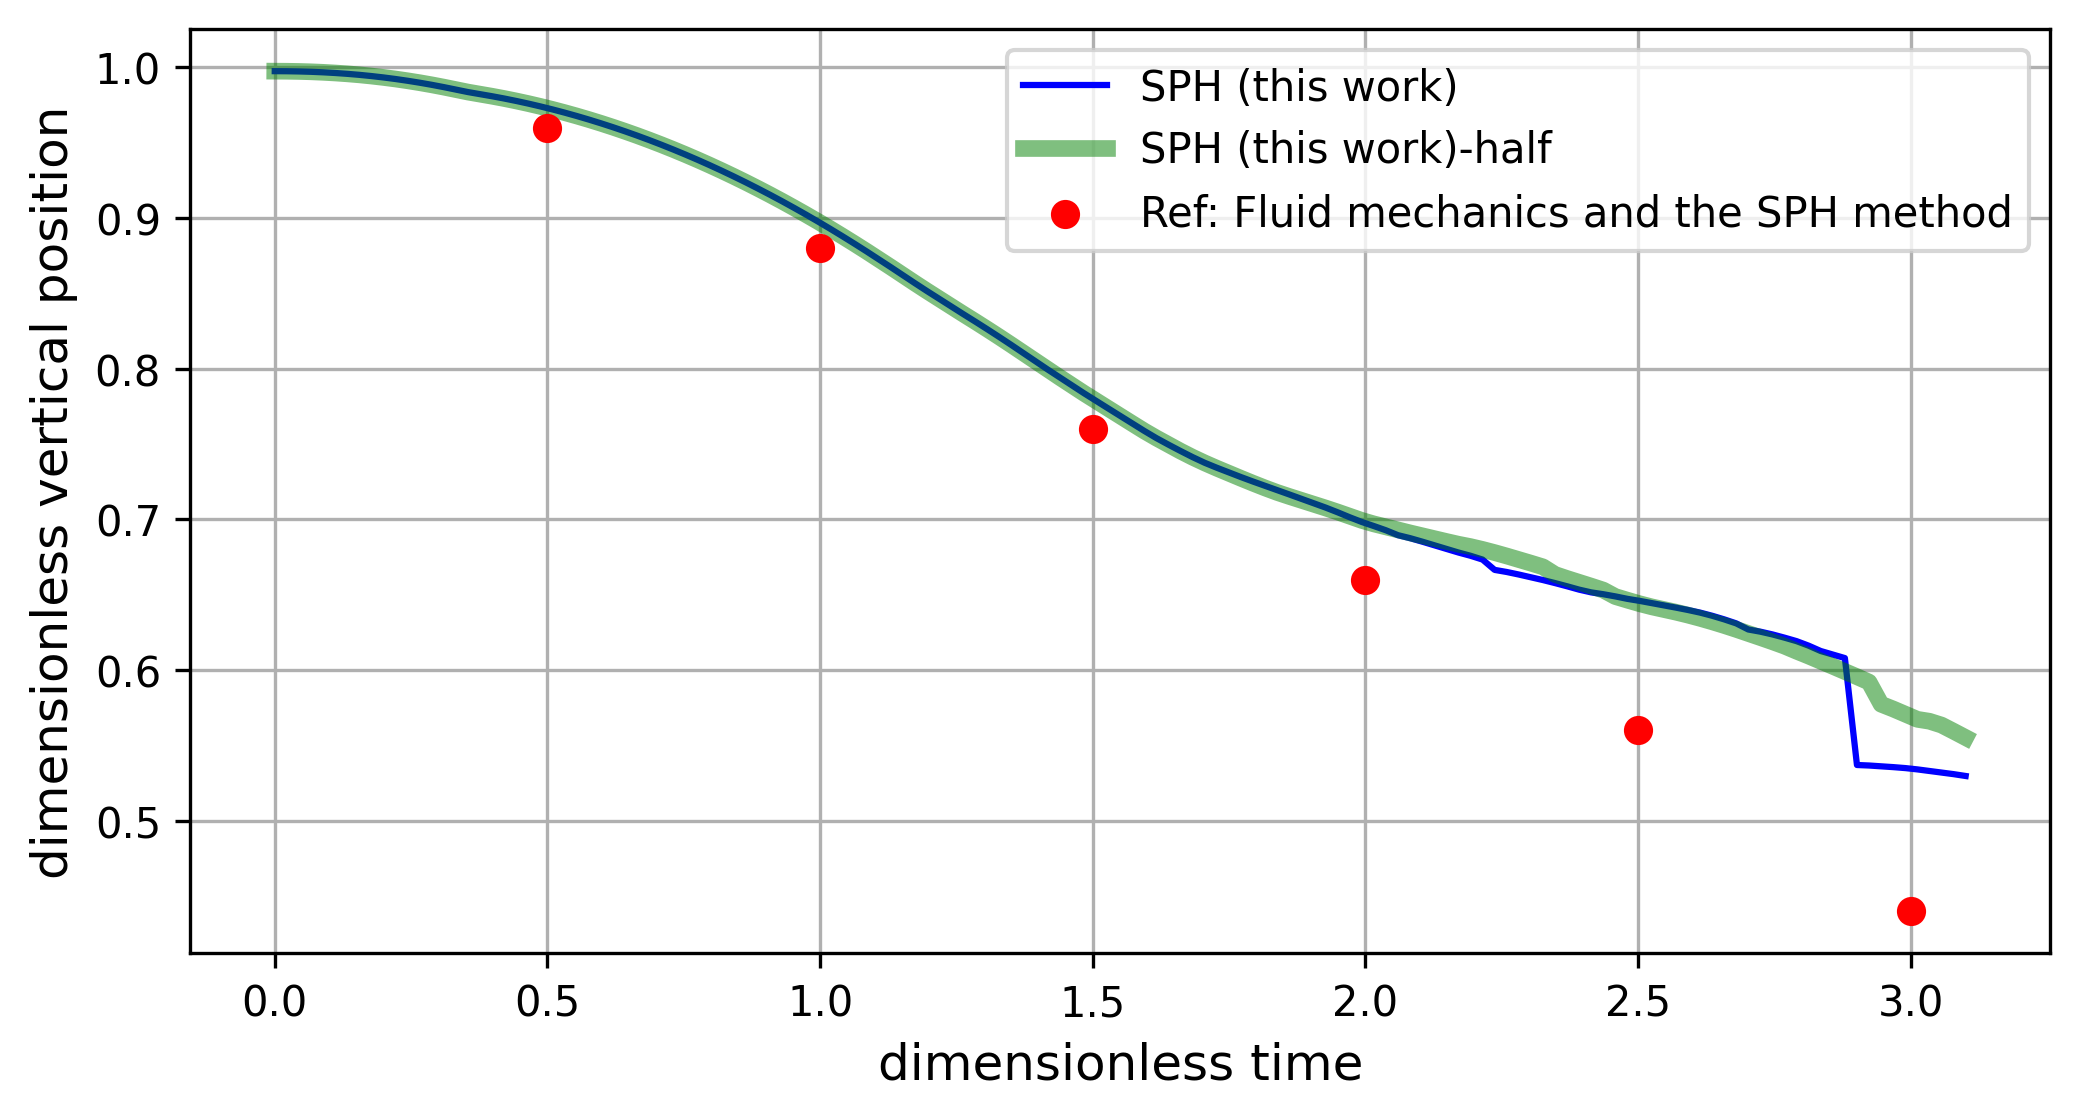
\includegraphics[width=\textwidth]{images/CollapseDry/vertical_position.png}
    \end{figure}
\end{frame}